% Created 2021-01-04 Mon 17:09
% Intended LaTeX compiler: pdflatex
\documentclass[10pt, a4paper]{article}
\usepackage[utf8]{inputenc}
\usepackage[T1]{fontenc}
\usepackage{graphicx}
\usepackage{grffile}
\usepackage{longtable}
\usepackage{wrapfig}
\usepackage{rotating}
\usepackage[normalem]{ulem}
\usepackage{amsmath}
\usepackage{textcomp}
\usepackage{amssymb}
\usepackage{capt-of}
\usepackage{hyperref}
\usepackage{titlesec}
\setcounter{secnumdepth}{4}
\titleformat{\paragraph}
{\normalfont\normalsize\bfseries}{\theparagraph}{1em}{}
\titlespacing*{\paragraph}
{0pt}{3.25ex plus 1ex minus .2ex}{1.5ex plus .2ex}
\usepackage[dvipsnames]{xcolor}
\usepackage{todonotes}
\usepackage{apacite}
\usepackage{lscape}
\usepackage[toc,page]{appendix}
\setlength{\parskip}{0.5em}
\hypersetup{colorlinks = true, linktocpage=true, filecolor = RoyalBlue, citecolor = RoyalBlue, linkcolor = RoyalBlue, urlcolor = RoyalBlue, unicode}
\setcounter{secnumdepth}{5}
\author{Njagi Mwaniki}
\date{\today}
\title{EXPLORING VIRUS SEQUENCE DIVERSITY USING GENOME GRAPHS}
\hypersetup{
 pdfauthor={Njagi Mwaniki},
 pdftitle={EXPLORING VIRUS SEQUENCE DIVERSITY USING GENOME GRAPHS},
 pdfkeywords={},
 pdfsubject={},
 pdfcreator={Emacs 27.1 (Org mode 9.4)}, 
 pdflang={English}}
\begin{document}

\begin{titlepage}
\centering
{\LARGE EXPLORING VIRUS SEQUENCE DIVERSITY USING GENOME GRAPHS \par }
\vspace {8cm}
{\small Njagi Mwaniki \par}
\vspace {8cm} 
{\small A thesis submitted in partial fulfilment of the             requirements for the award of a Master of Science Degree in             Bioinformatics of Pwani University. \par}
\vspace {1mm} 
{\small \today. \par}
\end{titlepage}
\urlstyle{same}
\newcommand{\bigO}{\mathcal{O}}

\pagenumbering{roman}

\setcounter{secnumdepth}{0}
\newpage

\section{Declaration}
\label{sec:orgc1542c3}
This thesis is my original work and has not been presented for a degree in any other university or any other award.

\vspace{10mm}

Moses Njagi Mwaniki

Date …………………………    Signature …………………….…………

\vspace{20mm}
I confirm that the work reported in this thesis was carried out by the candidate under my supervision.

\vspace{10mm}

Dr George Githinji

Date …………………………    Signature …………………….…………

\vspace{10mm}

Dr Pjotr Prins

Date …………………………    Signature …………………….…………

\vspace{10mm}

Prof James Nokes

Date …………………………    Signature …………………….…………


\newpage

\section{Dedication}
\label{sec:org3782075}
To my family, friends, mentors, and all the people whom this work will inform.

\newpage
\section{Acknowledgement}
\label{sec:orgdd3736b}
I would like to express my most profound appreciation to my supervisors
Dr George Githinji and Dr Pjotr Prins and Prof James Nokes, who introduced me to
the world of bioinformatics and more specifically genome graphs. Had it not been
for these people, this work would not be in existence.

It would also have been impossible to do without direction and guidance from
Erik Garrison, who has so eagerly walked me through the maze of graphical
pangenomics for over a year now. Friends like Christian Fischer, your help has
not gone unnoticed. The entire pantograph team that I worked with over the
virtual biohackathon gave me a great view of the world of graph visualisation.

KEMRI-Wellcome Trust and IDeAL for funding and facilitating this research
project and members of the IDeAL team (Prof Sam Kinyanjui, Dr Dorcas Mbuvi,
Liz Murabu, Solomon Mutuku, Rita Baya and Florence Kirimi) who patiently
followed up to know that everything was working great. My mates in the 2019/2020
IDEAL cohort who were a joy to be around and learn from.

Pwani University has been home for me for the last two years, the people there
are just the nicest people I have met. Prof Santi de Villiers has been
instrumental in guiding me through the masters and letting me know about
opportunities and understand the world of biology.
Prof. Suhaila Hashim for maintaining a great relationship with her students and
being so willing to help. My course-mates at Pwani University with whom we have
taken this bioinformatics journey for the last two years.

\textcolor{gray}{\emph{
“This work was supported through the DELTAS Africa Initiative [DEL-15-003].
The DELTAS Africa Initiative is an independent funding scheme of the
African Academy of Sciences (AAS)'s Alliance for Accelerating Excellence in
Science in Africa (AESA) and supported by the New Partnership for Africa's
Development Planning and Coordinating Agency (NEPAD Agency) with funding from
the Wellcome Trust [107769/Z/10/Z] and the UK government.
The views expressed in this publication are those of the author(s) and not
necessarily those of AAS, NEPAD Agency, Wellcome Trust or the UK government”.
}}

\newpage
\pagewidth
\section{Abstract}
\label{sec:org795d807}
\begin{ABSTRACT}
Linear reference genomes are a consensus of the most frequent base at a given
position.
Graph-based reference genomes represent a genome as a network of alternative
paths, thereby providing information on variant bases.
This graph can be node labelled—bases are held in the nodes of the graph while
the edges represent the connections between the bases, or edge labelled—if the
edges in the graph represent the bases. A graph-based data structure like this
is suitable for exploring and describing virus sequence diversity.
\todo{This last sentence can be better}

Sequenced respiratory syncytial virus raw reads from a twenty-five-member
household collected during a household outbreak were used to generate a genome
graph.
The sample reads were then aligned to the genome graph.
The number of reads that mapped under each node was then summarised as a
multidimensional coverage vector.
A pairwise Euclidean distance matrix of was computed and a neighbour-joining
cladogram based on hierarchical clustering generated.

We demonstrate the plausibility of differentiating a large number of closely
related consensus genomes by comparing the number of respective raw reads that
align to each node from the larger genome graph.
Additionally, the sequence coverage across a genome graph provides an
alternative approach for examining sequence relatedness and identifying
potential sequencing errors.
\end{ABSTRACT}
\setcounter{secnumdepth}{4}

\newpage

\setcounter{tocdepth}{5}
\tableofcontents


\newpage
\listoftables

\newpage
\listoffigures


\newpage
\pagenumbering{arabic}

\section{Introduction}
\label{sec:org0bbfdd5}
\subsection{Background Information}
\label{sec:org3365102}

Respiratory syncytial virus (RSV) was initially identified in Chimpanzees in
1956 and named Chimpanzee Coryza Agent \cite{morrisRecoveryCytopathogenicAgent1956}.
RSV was then isolated from children in 1957, from whom it had not been possible
to isolate, and renamed Respiratory Syncytial Virus to reflect the syncytia
which the virus caused to form in the tissue culture
\cite{chanockRecoveryInfantsRespiratory1957,beemAssociationChimpanzeeCoryza1960,falseyRespiratorySyncytialVirus2000}.

RSV produces an annual epidemic of predominantly upper respiratory tract
infections in children and healthy adults with re-infections occurring throughout
life even in the presence of pre-existing antibodies
\cite{nyiroDefiningVaccinationWindow2017,munoz-escalanteRespiratorySyncytialVirus2019,namRespiratorySyncytialVirus2019}.

It is the predominant viral cause of children admitted with severe pneumonia
\cite{berkleyViralEtiologySevere2010}
—the leading cause of childhood death in sub-Saharan Africa.
Further, it is the most frequent cause of acute lower respiratory tract
infection during the first year of life bringing infants between one and six
months of age into the hospital with pneumonia, bronchitis, otitis and increases
the prevalence of asthma amongst children hospitalised with RSV in infancy or
early childhood
\cite{borchersRespiratorySyncytialVirus2013,zlatevaMolecularEvolutionCirculation2004}.

\cite{nokesIncidenceSeverityRespiratory2009} proposed an effective pediatric
vaccine as the best way to prevent a sizable proportion of hospital admissions
attributable to pneumonia.
Looking into RSV prevention through immunisation
\cite{nyiroDefiningVaccinationWindow2017} used samples from the Kilifi pediatric
ward of children aged one day to less than twelve years.
They found that the presence of maternal antibodies in infants is highest at
birth and declines rapidly over the first six months of life.
Immunity was lowest between the ages of five to eleven months, meaning the span
between five and six months is the optimal time to vaccinate the infant.
However, a successful vaccine for children in this age range is yet to be
developed.

Among the elderly and high-risk immunocompromised adults, a simple upper
respiratory illness is no longer considered trivial.
People with cardiopulmonary diseases, cancer patients undergoing chemotherapy,
or those undergoing bone-marrow engraftment are at highest risk of pneumonia and
death.
For cancer patients, the risks and benefits of administering intensive
chemotherapy in the setting of a seemingly mild upper respiratory illness are
now weighed heavily
\cite{falseyRespiratorySyncytialVirus2000,whimbeyRespiratorySyncytialVirus2000}.

As of November 2020, linear references are the most popular medium used to
represent genomes—including the genome of RSV. There are, however, other ways of
representing a reference genome. Graph-based reference genomes,  unlike linear
references, represent a genome as a network containing alternative paths, and as
a consequence, aptly represent variation \cite{patenGenomeGraphsEvolution2017}.

Using graph-based genomes, we can use alternative nodes to represent alternative
alleles, mutations and other forms of variation in a genome.
By leveraging multiple paths, it has been possible to build tools which have
improved read mapping capability
\cite{garrisonVariationGraphToolkit2018,eizengaSuccinctDynamicVariation2020}.
We then can leverage this improved mapping capability to achieve a higher
resolution view into a genome and how it is changing. For this study it gives us
a better understanding of how the RSV genome is changing within or between hosts
over time.

\subsection{Problem Statement}
\label{sec:orgc1f5445}
As of November 2020, there has not been a successful RSV vaccine for children
between 0-2 months or even six months of age: the group in which RSV mortality
is highest \cite{nokesNewStrategiesControl2008}.
The lack of a viable preventive measure has led to the suggestion of cocooning,
an immunisation strategy which involves vaccinating the members of the household
that are most likely to transmit RSV to the infant
\cite{grizasCocooningConceptProtect2012,urwylerProtectingNewbornsPertussis2014,blainAssessmentCocooningStrategy2016}.
Cocooning thus depends on understanding who acquires the infection from whom
within the household.

By being a single path through a genome, linear references do not provide
sufficient resolution to fully reconstruct within-household transmission chains
\cite{agotiGenomicAnalysisRespiratory2019,githinjiAssessingUtilityMinority2018}.
Linear references from closely related samples such as those from the members of
a single household are too similar there causing phylogenetic methods to fail in
identifying transmission patterns based on the genomic data because there is not
sufficient phylogenetic and temporal signal. Besides, changes can arise due to
homoplasy and therefore are meaningless in inferring transmission.
According to \cite{agotiGenomicAnalysisRespiratory2019}, it was not possible to
determine who infects the infant in the household and come up with an effective
strategy for cocooning using alignment to linear references.

\subsection{Justification}
\label{sec:org29580d0}
A graph-based reference genome represents genomic variation as a network
structure where nucleotides are represented as nodes.
Variant nucleotides are represented as alternative nodes in the network.
Identical nucleotides are collapsed into a single node; implicitly encoding
genetic variation.
A linear reference genome, however, collapses these regions of diversity into a
single site based on the frequency of the bases at that given position.
We want to make use of genome graphs to understand the sequence diversity
present in RSV sequences, and potentially other respiratory viruses.

\newpage
\subsection{Objectives}
\label{sec:org632f81a}
\subsubsection{Main Objective}
\label{sec:orge598cbb}
To construct an RSV variation graph from RSV samples collected from a single
household in the course of a household RSV outbreak.

\subsubsection{Specific Objectives}
\label{sec:org856c953}
\begin{enumerate}
\item To assemble an RSV reference variation graph.
\item To use the reference variation graph assembled in the previous step to
compare the samples in the household RSV outbreak.
\end{enumerate}
\newpage
\section{Literature Review}
\label{sec:org69e18c0}
\subsection{RNA Viruses}
\label{sec:orgb8b3fc1}
In stark contrast with most organisms which exist distinct individuals with a
single genome; RNA viral populations exist as a quasispecies (also called a
mutant spectrum or a mutant cloud) where most of the biologically relevant
variation observed in vivo is as a result of genetic variation, competitive
selection and random events acting on multiple replicative units.
These quasispecies dynamics have been used to explain the failure of monotherapy
and synthetic antiviral vaccines but have opened new possibilities for antiviral
interventions \cite{domingoViralQuasispeciesEvolution2012}.

RNA viruses have mutation rates up to a million times higher than their hosts;
rates that are so high it is unlikely for a virus to have an identical RNA
molecule as its immediate progeny \cite{domingoViralQuasispeciesEvolution2012}.
Their mutation rate is not optimised by natural selection but instead is
controlled by negative selection with the proof being that their mutation
sometimes leads to local extinction \cite{duffyWhyAreRNA2018}.

\subsection{Respiratory Syncytial Virus (RSV)}
\label{sec:org7bd1f51}
RSV is the primary cause of acute lower respiratory tract infections associated
with pneumonia, bronchitis, and otitis
\cite{borchersRespiratorySyncytialVirus2013,kleinRoleRespiratorySyncytial1982,zlatevaMolecularEvolutionCirculation2004}
more frequently than any other agent and particularly in the first year of life
\cite{stottRespiratorySyncytialVirus1985}.
RSV significantly increases the prevalence of asthma in children hospitalised
with it \cite{saglaniViralInfectionsDevelopment2013}.

A mild upper respiratory illness in immunocompromised adults or the elderly is
no longer considered trivial \cite{whimbeyRespiratorySyncytialVirus2000}.
People with cardiopulmonary diseases and immunocompromised persons with bone
marrow transplant patients before marrow engraftment are at highest risk for
pneumonia and death \cite{morrisRecoveryCytopathogenicAgent1956}.
For cancer patients, the risks and benefits of administering intensive
chemotherapy in the setting of a seemingly mild upper respiratory illness are
now weighed heavily \cite{kleinRoleRespiratorySyncytial1982}.

\subsubsection{History}
\label{sec:orgdff3771}
The virus was first isolated in 1956 from Chimpanzees and named Chimpanzee
Coryza Agent \cite{morrisRecoveryCytopathogenicAgent1956}.
The next year, in 1957, it was isolated in
children from whom it had not been possible to isolate and renamed RSV and
classified in order Mononegavirales, family Paramyxoviridae, subfamily
Pneumovirinae, genus Pneumovirus
\cite{chanockRecoveryInfantsRespiratory1957,beemAssociationChimpanzeeCoryza1960,zlatevaGeneticVariabilityMolecular2005}.

\newpage

\subsubsection{Genetic Makeup}
\label{sec:orgfdede1a}
\begin{figure*}[h!]
\centering
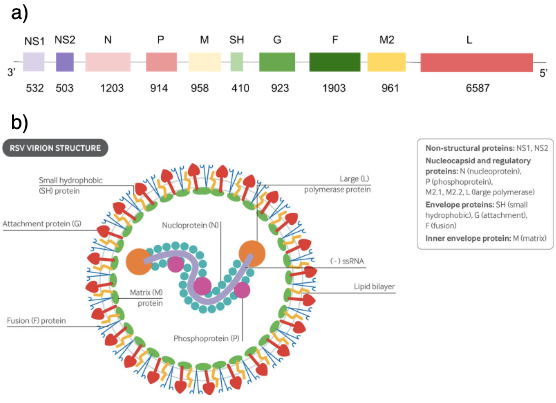
\includegraphics[width=1.0\textwidth]{../Figures/Schematic of RSV.png}
\caption[RSV Capsid]{\label{fig:org069c02c}(a) A schematic of RSV antisense RNA strand showing its ten genes. The rectangles represent genes with the different shades of the same colour used to show similarity. The grey connectors are the intergenic regions. The numbers below are the estimated gene lengths. (b) A schematic of the RSV capsid showing the lipid bilayer and most importantly, the surface of the F and G glycoproteins. Both images adapted from \cite{namRespiratorySyncytialVirus2019}.}
\end{figure*}

RSV, whose genome structure is shown in Figure \ref{fig:org069c02c}, is an enveloped virus with a
nonsegmented negative-strand RNA genome of approximately 15,200 nucleotides
containing ten genes which code for 11 proteins whose order is 3k NS1, NS2, N,
P, M1, SH, G, F, M2 (note that M2 codes for M2.1 and M2.2 proteins), and L with
attenuation of transcription step-wise with distance from the 3k end
\cite{caneMolecularEpidemiologyRespiratory2001}.

As shown in Table \ref{tab:orgb1a37c3} and Figure \ref{fig:org069c02c}, RSV has three surface glycoproteins: the small
hydrophobic (SH) protein which may be non-structural, the fusion (F) protein
which plays the leading role in virus penetration, syncytium formation, and
possibly can also mediate attachment and the attachment (G) glycoprotein which
plays the leading role in virus attachment. It has four nucleocapsid proteins
including the nucleoprotein (N), phosphoprotein (P), M2-1(also designated 22K
and sometimes considered a matrix protein) and polymerase (L).
The M2 gene contains a second open reading frame encoding a protein (M2-2)
which regulates transcription \cite{fearnsRoleM21Transcription1999}.
There is a single matrix protein, M1, which may mediate interactions between the
nucleocapsid and envelope and the two non-structural proteins, NS1 and NS2  have
recently been shown to antagonise the interferon-induced antiviral response
\cite{fearnsRoleM21Transcription1999,schlenderBovineRespiratorySyncytial2000}.



\begin{table}[htbp]
\centering
\begin{tabular}{lrl}
Gene & Approximate & Commentary\\
 & gene length in & \\
 & base pairs & \\
\hline
 &  & \\
\emph{Glycoproteins} &  & \\
F & 1903 & Virus penetration, syncytium\\
 &  & formation \& possibly mediate attachment\\
G & 923 & Mediate virus attachment\\
SH (1A) & 410 & Function unknown\\
 &  & \\
\emph{Membrane proteins} &  & \\
M & 958 & Basic; Transcription elongation factor\\
M2 (22K) & 961 & Basic; Regulation of transcription.\\
 &  & Codes for M2.2 and M2.1\\
 &  & \\
\emph{Nucleocapsid proteins} &  & \\
N & 1203 & Major nucleoplasmic protein\\
P & 914 & Acidic, phosphorylated\\
L & 6587 & Basic, hydrophobic, RNA polymerase\\
 &  & \\
\emph{Non-structural proteins} &  & \\
NS1 (1C) & 532 & Slightly acidic;\\
 &  & Antagonise interferon-induced antiviral response\\
NS2 (1B) & 503 & Basic\\
\end{tabular}
\caption[Summary of RSV Genes]{\label{tab:orgb1a37c3}A summary of RSV genes and their function. Listed are the glycoproteins (F, G, SH), membrane proteins (M, M2), nucleoplasmic proteins (N, P, L), non-structural proteins (NS1, NS2); their approximate lengths in base pairs and commentary on them.}

\end{table}



\subsubsection{Genetic Diversity}
\label{sec:orgc34dd46}
RSV was initially divided into two antigenic groups A and B in 1966 by its
reaction with panels of monoclonal antibodies particularly those directed
against its P, F and G proteins \cite{coatesAntigenicAnalysisRespiratory1966}.
It is worth noting that only antibodies directed against the G and F proteins
have been shown to be neutralising in vitro or protective in vivo. 

It was later demonstrated that the two groups are distinct at the genetic level.
The F and N proteins are highly conserved between the groups showing 91\% and 96\%
amino acid similarity, respectively
\cite{caneMolecularEpidemiologyRespiratory2001}.
In contrast, the G protein was found to be highly variable where the amino acid
similarity of this protein between groups A and B was 53\%
\cite{zlatevaMolecularEvolutionCirculation2004}.

Both groups are known to circulate within an epidemic
\cite{aamirMolecularCharacterizationCirculating2013}
without any leading to the extinction of the other, although A tends to be more
dominant in epidemics attributed to the higher variability among the A strains
\cite{zlatevaMolecularEvolutionCirculation2004,aamirMolecularCharacterizationCirculating2013}.

The sequence diversity of the G glycoprotein
(the type II glycoprotein of 289–299 amino acids depending on the virus strain
\cite{caneMolecularEpidemiologyRespiratory2001}
coded by the G gene suggests that the two subgroups have evolved
separately for a significant period of time with proof of RSV A’s most recent
common ancestor dating back as the early 1940s
\cite{zlatevaMolecularEvolutionCirculation2004}.

Because the F gene mutates at a much lower rate compared to the G gene, it
becomes an adequate vaccine target which is why we talk of RSV F vaccines
\cite{andersonStrategicPrioritiesRespiratory2013a,giersingReportWorldHealth2016}.
This lower rate of mutation also leads to consistent identification by
antibodies, and therefore the primary neutralising antibody response to RSV
appears to be induced by the F protein \cite{higginsAdvancesRSVVaccine2016}.

Groups A and B are subdivided further into subgroups based on differences in
their genomes.
As of 2012, there were 11 subgroups of RSV A: ON1, GA1–GA7, SAA1, NA1, and NA2
and 17 subgroups of RSV B: GB1–GB4, SAB1-SAB3, and BA1–BA10
\cite{aamirMolecularCharacterizationCirculating2013,eshaghiGeneticVariabilityHuman2012,peretCirculationPatternsGroup2000,trentoMajorChangesProtein2003,venterGeneticDiversityMolecular2001}.

Even with the existing classifications of RSV in their respective subgroups,
clear criteria for classifying RSV into subgroups is yet to be established
\cite{munoz-escalanteRespiratorySyncytialVirus2019}.
Because the G gene shows the highest variability, sufficient for strain
classification, little attention has been paid to the other viral genes
\cite{munoz-escalanteRespiratorySyncytialVirus2019}.
Classifying disease virulence by genotypes gives conflicting results in that a
strain which may seem to be virulent at a given time or place may seem to be
quite the opposite at a different time and place.
Thus suggesting the variations in other genes may contribute to strain virulence
and to epidemiological circulation patterns through time
\cite{andersonRSVStrainsDisease2019}.
Genome graphs which can allow for comparing entire genomes would provide a
better way of identifying how other genes affect virulence and epidemiological
circulation.

\subsubsection{Epidemiology}
\label{sec:org02f5516}
In older children and healthy adults, RSV presents in highly seasonal annual
epidemics \cite{al-toumEpidemiologyClinicalCharacteristics2006,aamirMolecularCharacterizationCirculating2013}
of mild reinfections predominantly in the upper respiratory tract even in the presence
of pre-existing antibodies
\cite{sullenderGeneticDiversityAttachment1991,caneMolecularEpidemiologyRespiratory2001}.
The epidemics have been found to have a significant negative correlation with
temperature and a significant positive correlation with relative humidity and
rainfall \cite{al-toumEpidemiologyClinicalCharacteristics2006} and therefore crop
up in the coldest months which naturally vary with latitude.

Critical illness of RSV is limited to the primary infection which occurs
between six weeks and two years of age during the child’s first or second
epidemics \cite{caneMolecularEpidemiologyRespiratory2001} and can occur in the
presence of maternally derived antibodies which are present up to five months of
age \cite{nyiroDefiningVaccinationWindow2017}.
However, infants with more severe illnesses were found to have lower levels of
antibodies in serum collected near the onset of disease than did infants with
milder illnesses \cite{caneMolecularEpidemiologyRespiratory2001}.

In temperate climates, RSV epidemics occur in the winter between December and
February but peaking in January and February \cite{al-toumEpidemiologyClinicalCharacteristics2006}
and are a significant cause of winter mortality associated with 60-80\% more
deaths than influenza \cite{nicholsonImpactInfluenzaRespiratory1996}.
In tropical climates, epidemics occur during the rainy season
\cite{al-toumEpidemiologyClinicalCharacteristics2006,aamirMolecularCharacterizationCirculating2013}
but are also associated with religious festivals
\cite{caneMolecularEpidemiologyRespiratory2001}.

In Italy, \cite{rossiRiskFactorsSevere2007}, showed that an infant having siblings was among
the risk factors that could lead to RSV inducing a Lower Respiratory Tract
Infection (LRTI) severe enough to lead to hospital admission.
The study also found that being at least the second child to be a risk factor
for severe RSV induced LRTI. 

In Kilifi, \cite{nokesIncidenceSeverityRespiratory2009},
found that RSV epidemics do not have a simple annual pattern but rather an
interepidemic period alternating between 9 and 15 months.
They do however start from November through February and peak from January
through May.
A different study in Kilifi, \cite{okiroFactorsAssociatedIncreased2008}, found
that household crowding, which is assumed to increase contact intensity
resulting in increased duration of exposure led to higher rates of RSV infection
in infants.

A key target group for an RSV pediatric vaccine is infants under two months of
age \cite{nokesNewStrategiesControl2008}; however, vaccine development has been
unsuccessful for young infants around this age.
In contrast, this has not been the case for older children. Mathematical models
\cite{whiteTransmissionDynamicsGroups2005,whiteUnderstandingTransmissionDynamics2007}
suggest that vaccination of older infants or siblings
could be pivotal in avoiding infection for younger children.
In Kilifi, \cite{kinyanjuiVaccineInducedHerd2015,munywokiInfluenceAgeSeverity2015}
found that immunisation of young children between five to ten months is likely
to be a highly effective method for protection of infants below three months of
age.

A method of indirect protection of young infants through the immunisation of
older members of the household, cocooning, is necessary to interrupt chains of
transmission; therefore, providing indirect protection to infants.
It is crucial to determine from whom infants acquire their infection from to
determine who is best to target for immunisation—especially given the budget
constraints in developing countries.

\newpage

\subsection{The Kilifi Household Study}
\label{sec:org958cee9}
The home is where infants spend most of their time, on top of that, households
are areas of frequent and intense contact—conducive for the spread of
respiratory viruses, including RSV. In 2010 Muywoki et al. developed a
prospective study to investigate the introduction and transmission of RSV in
households using molecular techniques. The primary objective of this study was
to determine who acquires infection from whom (WAIFW) within households during
RSV outbreaks \cite{munywokiTransmissionRespiratorySyncytial2013}.
This study was carried out in the Matsangoni location, within the Kilifi Health
and Demographic Surveillance System \cite{scottProfileKilifiHealth2012},
Kilifi District, Kenya during the RSV season between November 2009 and
June 2010. In addition, the study area has six public primary schools and one
non-boarding secondary school.

The study involved 493 members of 47 households. Each household had to have an
infant, a member of the household below one year of age, born after the previous
RSV epidemic and at least one elder sibling. Nasopharyngeal (NSP) swabs were
collected every 3-4 days irrespective of symptoms and tested for respiratory
viruses, including RSV, using a molecular diagnostic assay. Moreover, once a
week, a specimen of oral fluid from around the gums was collected for RSV
antibody screening and sensitivity of oral fluid (OF) detection of RSV in
molecular diagnostics.
A total of 16, 924 NPS swabs were collected, representing 86\% of the planned
\cite{munywokiTransmissionRespiratorySyncytial2013}.

A whole-genome sequencing (WGS) assay for RSV was developed with the aim of
resolving chains of transmission within the household, and to study rates of
mutation and minor-variant population dynamics within and between infected hosts
\cite{agotiGeneticDiversityRespiratory2014}.
RSV was detected in 40 (85\%) households and 179 (36\%) of the participants.
In 28 of the 44 households with complete data, there was transmission of RSV to
the infants experiencing their first epidemic
\cite{munywokiTransmissionRespiratorySyncytial2013}.
This study thus provided suitable samples to analyse how RSV is transmitted
within the community, schools and, for our purposes, the home
\cite{agotiTransmissionPatternsEvolution2017,agotiGenomicAnalysisRespiratory2019,githinjiAssessingUtilityMinority2018,kinyanjuiVaccineInducedHerd2015,munywokiInfluenceAgeSeverity2015}. 

To focus the study on household transmission, I focused on samples from a single
household, HH5, which was a large household of twenty-five members with an
infant and school-going siblings and genetically closely related samples going
by previous studies
\cite{githinjiAssessingUtilityMinority2018,agotiGenomicAnalysisRespiratory2019}.


\newpage

\subsection{Graphs in Bioinformatics}
\label{sec:org7b2ba71}
Contemporary reference genomes utilise a linear sequence of characters to
represent the bases that make up the DNA of multiple individuals, shown in
Figure \ref{fig:org5adc1e2}.
This linearity introduces a bias in mapping known as reference bias
\cite{degnerEffectReadmappingBiases2009,diltheyImprovedGenomeInference2015}.

Reference bias is a tendency in read mapping to overlook variation and
overreport sequence that is present in the reference compared to the sequence
that is not present in the reference.
This bias is exacerbated in reads which are highly divergent from the reference,
such as structural variation, or which are completely absent from the reference
\cite{degnerEffectReadmappingBiases2009,schneebergerSimultaneousAlignmentShort2009,liBuildingSequenceMap2010,brandtMappingBiasOverestimates2015,patenGenomeGraphsEvolution2017,garrisonVariationGraphToolkit2018}.

\begin{figure}[htbp]
\centering
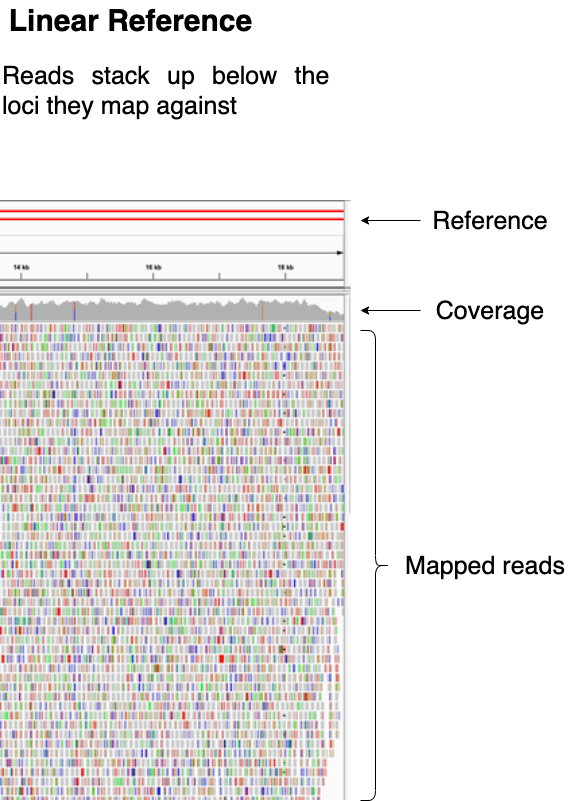
\includegraphics[width=0.75\textwidth]{../Figures/Alignment-igv.png}
\caption[Read alignment against a linear reference]{\label{fig:org5adc1e2}A screenshot of reads aligned to a linear reference in igv.}
\end{figure}


The inability of linear references to hold information on genetic variation has
led to the need for a structure that can represent variation that is inherent in
the genome.
Other models, such as the variant-call format to hold variation information, or
assembly graphs often represented as FASTG or GFA, can approach this structure
with varying degrees of accuracy but they are decoupled from the reference and
therefore not incorporated in mapping and consequently the comparison of
samples. 

Graph structures, on the other hand, are malleable, can be updated, and can
comfortably represent contradicting information, as alternative nodes, allowing
them to straightforwardly represent a genome and its inherent variation
\cite{patenGenomeGraphsEvolution2017,liDesignConstructionReference2020}.
Graphical representation of the reference sequence will expectedly lead to
improvements in mapping reads, variant calling and haplotype determination
\cite{patenGenomeGraphsEvolution2017}.
This is facilitated by the increased resolution in read mapping provided by
genome graphs Figure fig:alignment-graphical.

\begin{figure}[htbp]
\centering
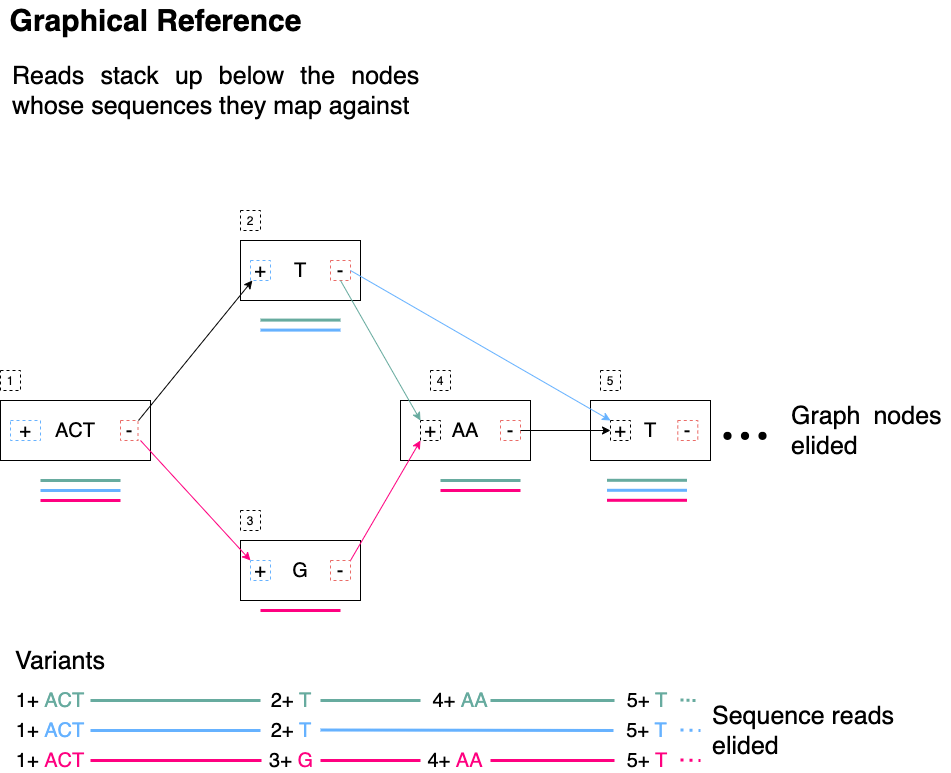
\includegraphics[width=0.75\textwidth]{../Figures/Alignment-graph-schematic.png}
\caption[Read alignment against a graph-based reference]{\label{fig:org1e6aadc}A schematic of reads aligned against a graph.}
\end{figure}


Reference bias affects how samples are compared against each other in downstream
analysis leading to the need to draw out a representative structure that
accounts for variation using which samples can be compared—Figure
\ref{fig:org1e6aadc}.
This representative structure, in our case, is a coverage vector.

\begin{figure}[htbp]
\centering
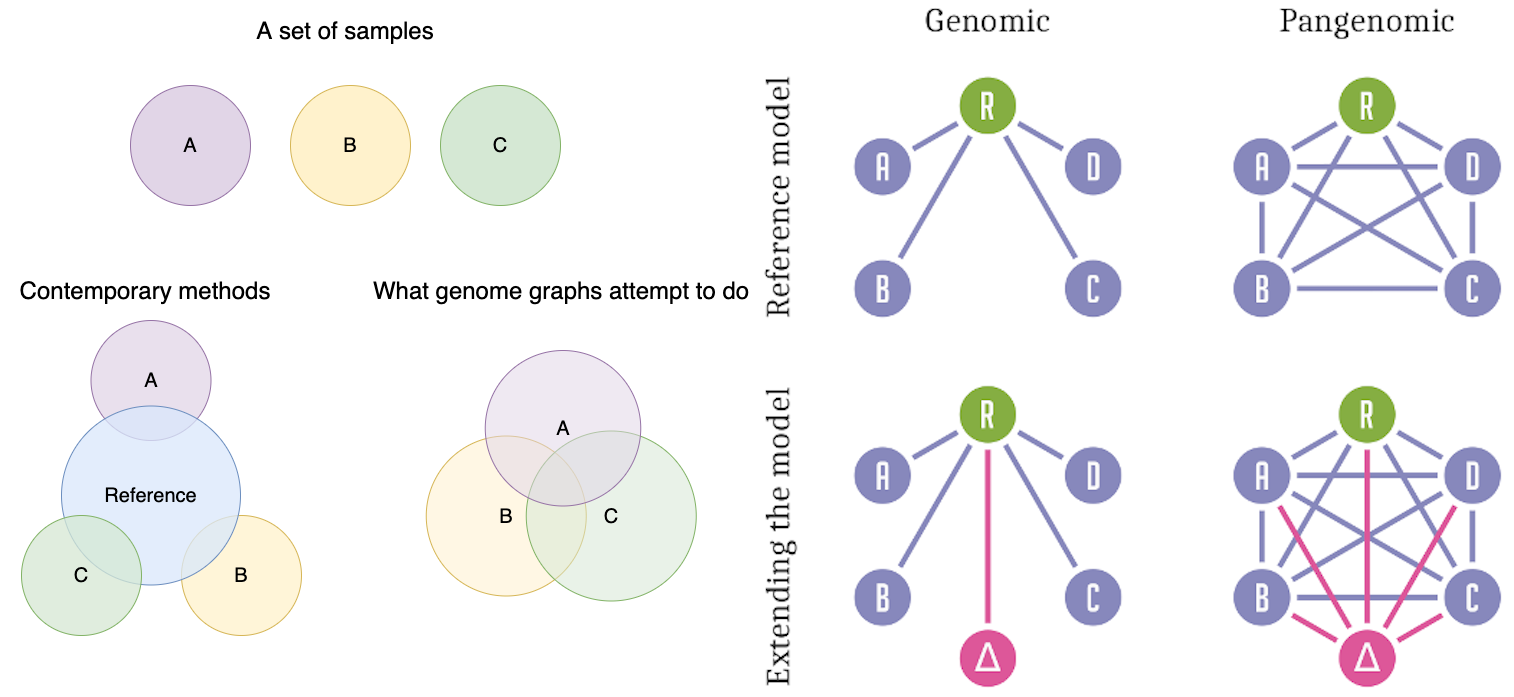
\includegraphics[width=0.75\textwidth]{../Figures/combined-all-vs-all.png}
\caption[Graphical all vs all comparison]{\label{fig:org607f8fe}Contemporary genomic methods compare each sample based on how it compares against a reference. A pangenomic method compares each sample against every other sample through the use of a reference pangenome graph. a) Shows this comparison using Venn diagrams and three samples A, B, and C. b) from \cite{eizengaSuccinctDynamicVariation2020}.}
\end{figure}


This study hypothesises that looking into genomic variation in the household
with the help of genome graphs will take us a step forward in understanding
household transmission, for which the tools we use today are not giving us
sufficient resolution.
The hope is that the previously demonstrated increased resolution by variation
graphs \cite{garrisonVariationGraphToolkit2018} will prove especially useful at
the level of the household.


\clearpage

\subsection{Graph Theory}
\label{sec:org22a28ba}
A graph is an object, or collection, of two sets, a vertex set and edge set.
The vertex set is a finite non-empty set. A graph must therefore have at least
one vertex.
The edge set may be empty \cite{trudeauIntroductionGraphTheory1993}
and is used to present relationships between the vertices.

Figure \ref{fig:org5388111} shows how a graph can be represented
visually.


\begin{figure*}[!ht]
\centering
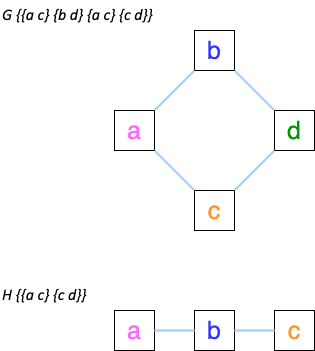
\includegraphics[width=0.5\textwidth]{../Figures/Three-and-four-node-graph.png}
\caption[A Three Node and A Four Node Graph]{\label{fig:org5388111}G is an undirected graph with four nodes a,b,c and d. H is an undirected graph with nodes a, b and c.}
\end{figure*}

\subsubsection{Classifications of Graphs}
\label{sec:orgbfa6c20}
Graphs can be broken down into many classifications, but in this case, we want
to focus on simple versus multigraphs and directed versus undirected.
A simple graph can only have one edge connecting two adjacent vertices while a
multigraph is a graph in which two adjacent vertices are connected by more than
one edge.

\begin{figure*}[!ht]
\centering
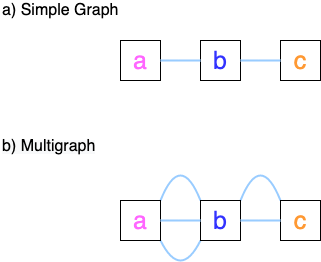
\includegraphics[width=0.6\textwidth]{../Figures/Simple-and-Multigraph.png}
\caption[A simple graph and a multigraph]{\label{fig:org7d8874c}(a) A diagram of a simple graph; any two nodes in such a graph are connected by a single edge. (b) A multigraph where more than one edge can connect any two nodes.}
\end{figure*}

A directed graph (Figure \ref{fig:org1f4ec0b}) also called a digraph is a graph in which the edges have
direction.

\begin{figure*}[!ht]
\centering
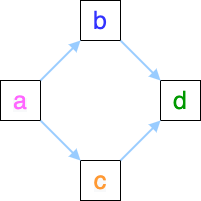
\includegraphics[width=0.4\textwidth]{../Figures/Digraph.png}
\caption[A Directed Graph]{\label{fig:org1f4ec0b}A directed graph with the edges indicating direction.}
\end{figure*}

An undirected graph (Figure \ref{fig:org8d6b2b8}) is one in which the edges do
not have direction indicated on them.

\begin{figure*}[!ht]
\centering
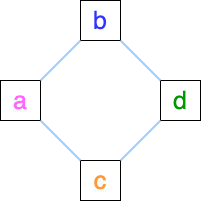
\includegraphics[width=0.4\textwidth]{../Figures/Undirected.png}
\caption[An Undirected Graph]{\label{fig:org8d6b2b8}An undirected graph where the edges have no indication of direction.}
\end{figure*}

A bidirected graph is one in which each edge has an independent orientation
\cite{edmondsMatchingWellSolvedClass2003}.
This is important for the representation of strand,
that is, reading a DNA molecule in its forward or reverse complement orientation
\cite{patenGenomeGraphsEvolution2017}.

The degree of a vertex v in a graph G, is the number of edges of G incident with
v (going in and out of v), each loop counting as two edges.
In directed graphs, we have the concept of indegree and outdegree.
The indegree refers to the numbers of head ends of the edges adjacent to a
vertex, and the outdegree is the number of tail ends of the edges adjacent to a
vertex \cite{bondyGraphTheory2011}. A vertex is even if its degree is an even number
and odd otherwise \cite{trudeauIntroductionGraphTheory1993}.

An isomorphism (Figure \ref{fig:orgcb3555f}) is a relationship between two graphs such
that the two graphs can be represented by identical diagrams
\cite{bondyGraphTheory2011}
whereas an automorphism of a graph is an isomorphism of the graph to itself as
shown below.

\begin{figure*}[h]
\centering
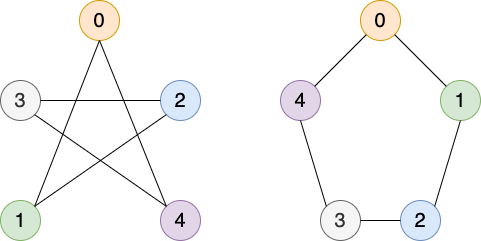
\includegraphics[width=0.6\textwidth]{../Figures/Isomorphism.png}
\caption[A graph isomorphism]{\label{fig:orgcb3555f}The two nodes are different visualizations of the same graph and therefore an isomorphism.}
\end{figure*}

\subsubsection{Walks and paths}
\label{sec:org9aa98b8}
A path is a simple graph whose vertices can be arranged in a linear sequence in
such a way that two vertices are adjacent if they are consecutive in the
sequence, and are nonadjacent otherwise \cite{bondyGraphTheory2011}.


A walk in a graph is a sequence  of not necessarily distinct vertices in which
A1 is joined by an edge to A2, A2 is joined by an edge to A3, \ldots{}, and An−1 is
joined by an edge to An. The walk is said to join A1 and An
\cite{trudeauIntroductionGraphTheory1993}.

Therefore, a path is a graph, whereas a walk is a traversal of a graph.

An Euler or Eulerian walk is a walk that uses every edge in the graph exactly
once.

A Hamiltonian walk is like an Eulerian walk, but for nodes and can be open or
closed, an open hamilton walk is a walk that uses every vertex in the graph
exactly once.
A closed hamilton walk is a closed walk that uses the initial vertex exactly
twice and all the other vertices in the graph exactly once
\cite{trudeauIntroductionGraphTheory1993}.

\newpage

\subsection{Pangenome Graphs}
\label{sec:org71236af}
Pan is a word that implies the combinations of many or all; therefore, a
pangenome is a genome that is composed of many or all genomes. Going by this, a
pangenome graph (closely related to a genome graph) is a genome graph capable of
representing a pangenome.
RNA viruses, given their quasispecies characteristic and small genome size,
lend themselves naturally to have their genomes represented as pangenomes.

Pangenome graphs can be broadly categorised into reference-guided and
reference-free (de novo) with some tools supporting both. De novo approaches do
not require any prior information, such as a reference genome or knowledge of
the quasispecies or pangenome composition. De novo approaches have been shown to
have advantages over reference-guided reconstruction, since using a reference
genome can induce significant biases \cite{baaijensStrainawareAssemblyGenomes2019}.

\subsubsection{Sequence graph}
\label{sec:org4b39031}
Sequence graphs, though not used in and of themselves, are built upon to
implement pangenome graphs.
A sequence graph, Figure 10, is a bidirected graph in which each node is
labelled with a nucleotide string \cite{patenGenomeGraphsEvolution2017}.
In this bidirected graph, the features of an edge indicate to which side of a
node (sequence), either 5’ or 3’, each end of the edge connects
\cite{novakGenomeGraphs2017}.


\begin{figure*}[h]
\centering
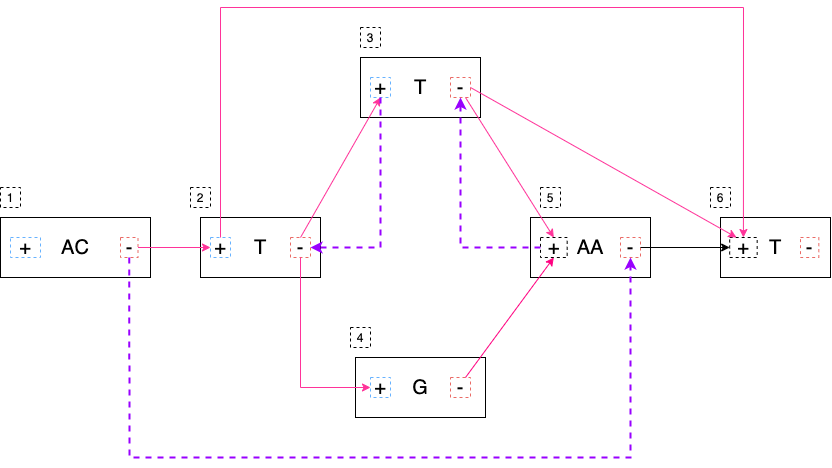
\includegraphics[width=0.75\textwidth]{../Figures/sequence-graph.png}
\caption[Sequence Graph]{\label{fig:org724e80a}A sequence graph where nodes are labelled with nucleotides and the edges encode strandedness of the nucleotide connection, which is forward or reverse. The forward strands are represented by pink edges while reverse strands are represented by dotted purple edges.}
\end{figure*}

\subsubsection{Variation Graph}
\label{sec:org62868e7}
A variation graph is a graph where a complete walk along the graph represents a
haplotype \cite{patenGenomeGraphsEvolution2017}. Variation graphs are genome
graphs that embed the paths in the graph \todo{Citation Needed}.
In the case of viruses, these paths can be used to represent unique viral
genomes in quasispecies, haplotypes. 

Many genome graphs do not represent the concept of the strand—reading a DNA
molecule in its forward and reverse complement orientations.
\cite{patenGenomeGraphsEvolution2017}. To express strandedness, directed graphs
can be generalised to bidirected graphs
\cite{edmondsMatchingWellSolvedClass2003,medvedevComputationalMethodsDiscovering2009}
in which each edge endpoint has an independent orientation, indicating whether
the forward or the reverse complement strand of the attached node is to be
visited when entering the node through that endpoint of the edge. Inversions,
reverse tandem duplications, and arbitrarily complex rearrangements are
expressible in the bidirected representation \cite{patenGenomeGraphsEvolution2017}.


\definecolor{mypink}{RGB}{225, 0, 128}
\definecolor{mygreen}{RGB}{106, 168, 79}
\definecolor{myblue}{RGB}{111, 168, 220}
\definecolor{myred}{RGB}{225, 0, 0}
\definecolor{mypurple}{RGB}{153, 0, 255}

\begin{center}
\begin{tabular}{llllllll}
\color{mypink}Individual 1 & \color{mypink} A & \color{mypink} C & \color{mypink} T & \color{mypink} G & \color{mypink} A & \color{mypink} A & \color{mypink} T\\
\color{myblue}Individual 2 & \color{myblue} A & \color{myblue} C & \color{myblue} T & \color{myblue} T & \color{myblue} - & \color{myblue} - & \color{myblue} T\\
\color{mygreen}Individual 3 & \color{mygreen} A & \color{mygreen} C & \color{mygreen} T & \color{mygreen} T & \color{mygreen} A & \color{mygreen} A & \color{mygreen} T\\
\hline
\color{red}Consensus & \color{red} A & \color{red} C & \color{red} T & \color{red} T & \color{red} A & \color{myred} A & \color{red} T\\
\end{tabular}

\end{center}


\begin{figure*}[h!]
\centering
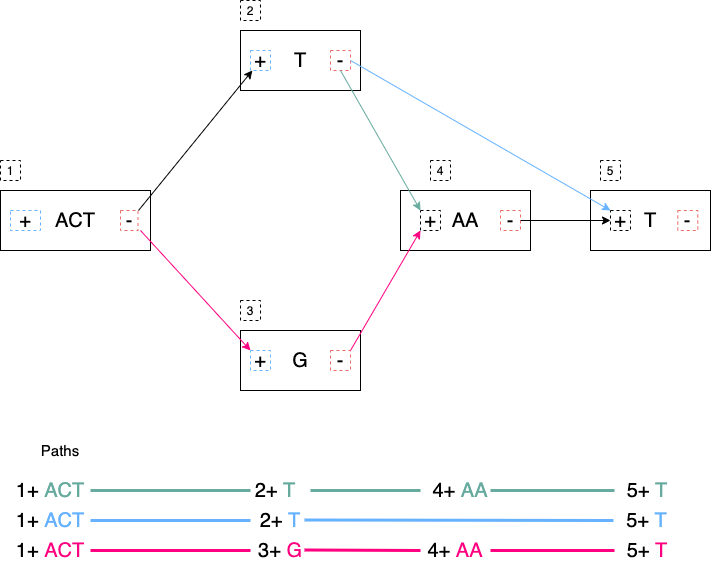
\includegraphics[width=0.7\textwidth]{./figures/Variation-Graph-Page-1.png}
\caption[Variation Graph]{\label{fig:orgade5fbb}A variation graph with the paths outlined at the bottom}
\end{figure*}


In case of addition of individual 4 containing an inversion at node 2,3 and 4


\begin{center}
\begin{tabular}{llllllll}
\color{mypink}Individual 1 & \color{mypink} A & \color{mypink} C & \color{mypink} T & \color{mypink} G & \color{mypink} A & \color{mypink} A & \color{mypink} T\\
\color{myblue}Individual 2 & \color{myblue} A & \color{myblue} C & \color{myblue} T & \color{myblue} T & \color{myblue} - & \color{myblue} - & \color{myblue} T\\
\color{mygreen}Individual 3 & \color{mygreen} A & \color{mygreen} C & \color{mygreen} T & \color{mygreen} T & \color{mygreen} A & \color{mygreen} A & \color{mygreen} T\\
\color{mypurple}Individual 4 & \color{mypurple} A & \color{mypurple} C & \color{mypurple} A & \color{mypurple} A & \color{mypurple} T & \color{mypurple} T & \color{mypurple} T\\
\hline
\color{red}Consensus & \color{red} A & \color{red} C & \color{red} T & \color{red} T & \color{red} A & \color{myred} A & \color{red} T\\
\end{tabular}

\end{center}


\begin{figure*}[h!]
\centering
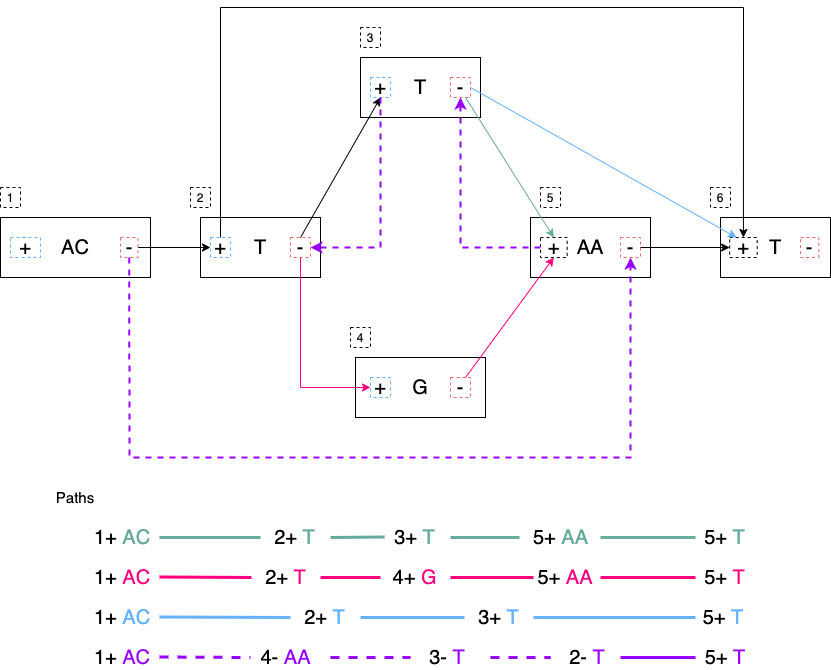
\includegraphics[width=0.7\textwidth]{./figures/Variation-Graph-Page-2.png}
\caption[Variation Graph with Inversion]{\label{fig:orgd07afad}A variation graph represeting the paths but containing an inversion in individual 4}
\end{figure*}


Compared to eukaryotes, viruses have relatively short genomes, and high
mutation rates \cite{duffyWhyAreRNA2018} and RNA viruses exist as a quasi-species
\cite{domingoViralQuasispeciesEvolution2012}.
This gives rise to the need to deconvolute the individual haplotypes and
quantify them, making variation graphs a prime instrument for this.
VG-flow \cite{baaijensStrainawareAssemblyGenomes2019} performs de novo, strain aware metagenomic
assembly focusing on short-read data.  It takes as input next-generation
sequencing (NGS) data and a collection of strain-specific contigs assembled from
the data and produces full-length haplotypes and corresponding abundance
estimates.

\subsubsection{Population Reference Graphs (PRGs)}
\label{sec:org113cb22}
Population reference graphs are graphs that represent a population-wide genome
combining multiple reference sequences and catalogues of variation
\cite{diltheyImprovedGenomeInference2015,liDesignConstructionReference2020}. 
This concept may also be extended to represent, in our case, a virus mutant
cloud.

\subsection{Problems arising from graph-based reference models}
\label{sec:orgee80533}
\subsubsection{Coordinate system}
\label{sec:org27e413e}
A reference genome coordinate system is a system that uniquely determines the
positions of bases in the reference genome 
\cite{randCoordinatesIntervalsGraphbased2017}. 
This is trivial with linear references where bases are ordered ascendingly from 
left to right, but with graphs, it is no longer trivial to define a locus on 
the reference \cite{patenGenomeGraphsEvolution2017}. 

According to the Computational Pan-Genomics Consortium (2016), there are three
qualities that a coordinate system should have 
\cite{patenGenomeGraphsEvolution2017,randCoordinatesIntervalsGraphbased2017}. 
A coordinate system should have: i) monotonicity genome graph coordinates of
successive bases within a genome should be increasing, ii) legibility
coordinates should be compact and human interpretable, and iii) spatiality
bases physically close together within a genome should have similar coordinates,
vertical spatiality of bases that are allelic variants of one another 
\cite{randCoordinatesIntervalsGraphbased2017} horizontal spatiality of bases that can appear together 
within a single molecule \cite{randCoordinatesIntervalsGraphbased2017}. 

The vg family of tools solves this through topological sort, which gives an 
ascending order of the nodes.

\subsubsection{Calling alleles at sites}
\label{sec:orgdbedd57}
Calling an allele is declaring its presence at a given position which could span
several nodes or edges in an undefined manner. 
A proposed way to describe their positions is via motif
\cite{patenGenomeGraphsEvolution2017}, patterns of interconnections occurring in
complex networks at numbers that are significantly higher than those in
randomised networks \cite{miloNetworkMotifsSimple2002}, called a superbubble in directed graph
or an ultrabubble in bidirected graphs \cite{patenGenomeGraphsEvolution2017}.
Superbubbles and ultrabubbles are directed acyclic subgraphs that connect to the
rest of the graph through one source node and one sink node
\cite{patenGenomeGraphsEvolution2017}.

\begin{figure*}[h]
\centering
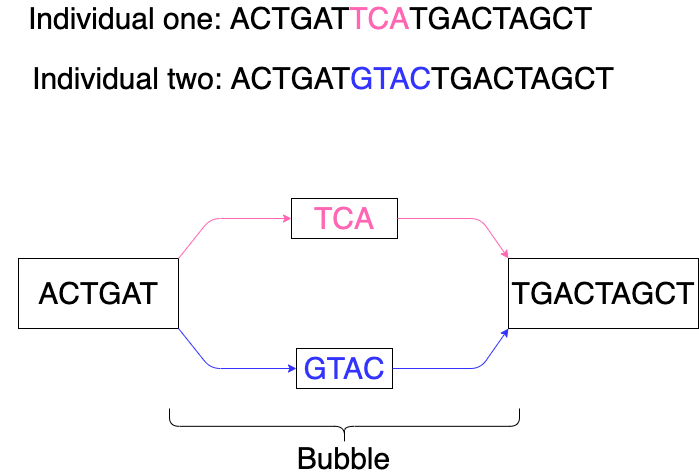
\includegraphics[width=0.75\textwidth]{../Figures/bubble.png}
\caption[A bubble in a graph]{\label{fig:orgefc6fda}A hypothetical genome graph constructed from the genomes of two individuals, one and two, with a bubble forming around the divergence between the two genomes.}
\end{figure*}

In this case, we could declare that an allele occurs in the bubble ranging from
a given start node to a given end node.

\subsubsection{Non-trivial indexing and reference mapping}
\label{sec:org77eaedd}
Genome graphs increase the amount and complexity of the text needed for search
problems. 
This means genome graph tools have to employ methods that are aware of 
alternative alleles as well as the increased number of paths 
\cite{patenGenomeGraphsEvolution2017}. 
The solution to this is contemporary indexing methods have to be generalised to 
graph structures; generalisations such as the gBWT (Sirén et al., 2018) could
 be achieved via partial order alignment GSSW \cite{zhaoSSWLibrarySIMD2013}.

\newpage
\section{Materials and Methods}
\label{sec:orgb4f65dc}
\subsection{RSV}
\label{sec:org5d8d3b8}
We started the experiment with fifty three whole genome sequenced RSV 
positive samples from a twenty five member household code-named household twenty
which was part of a household follow up study in the Kilifi Health and 
Demographic Surveillance System and ran over a six month
period collecting nasopharyngeal swabs twice each week
\cite{munywokiInfluenceAgeSeverity2015,agotiTransmissionPatternsEvolution2017,githinjiAssessingUtilityMinority2018}.

Figure \ref{fig:orgbba1b9e} from
\cite{githinjiAssessingUtilityMinority2018} shows the temporal infection patterns
of nineteen of the twenty five members of household twenty.

\begin{figure*}[h]
\centering
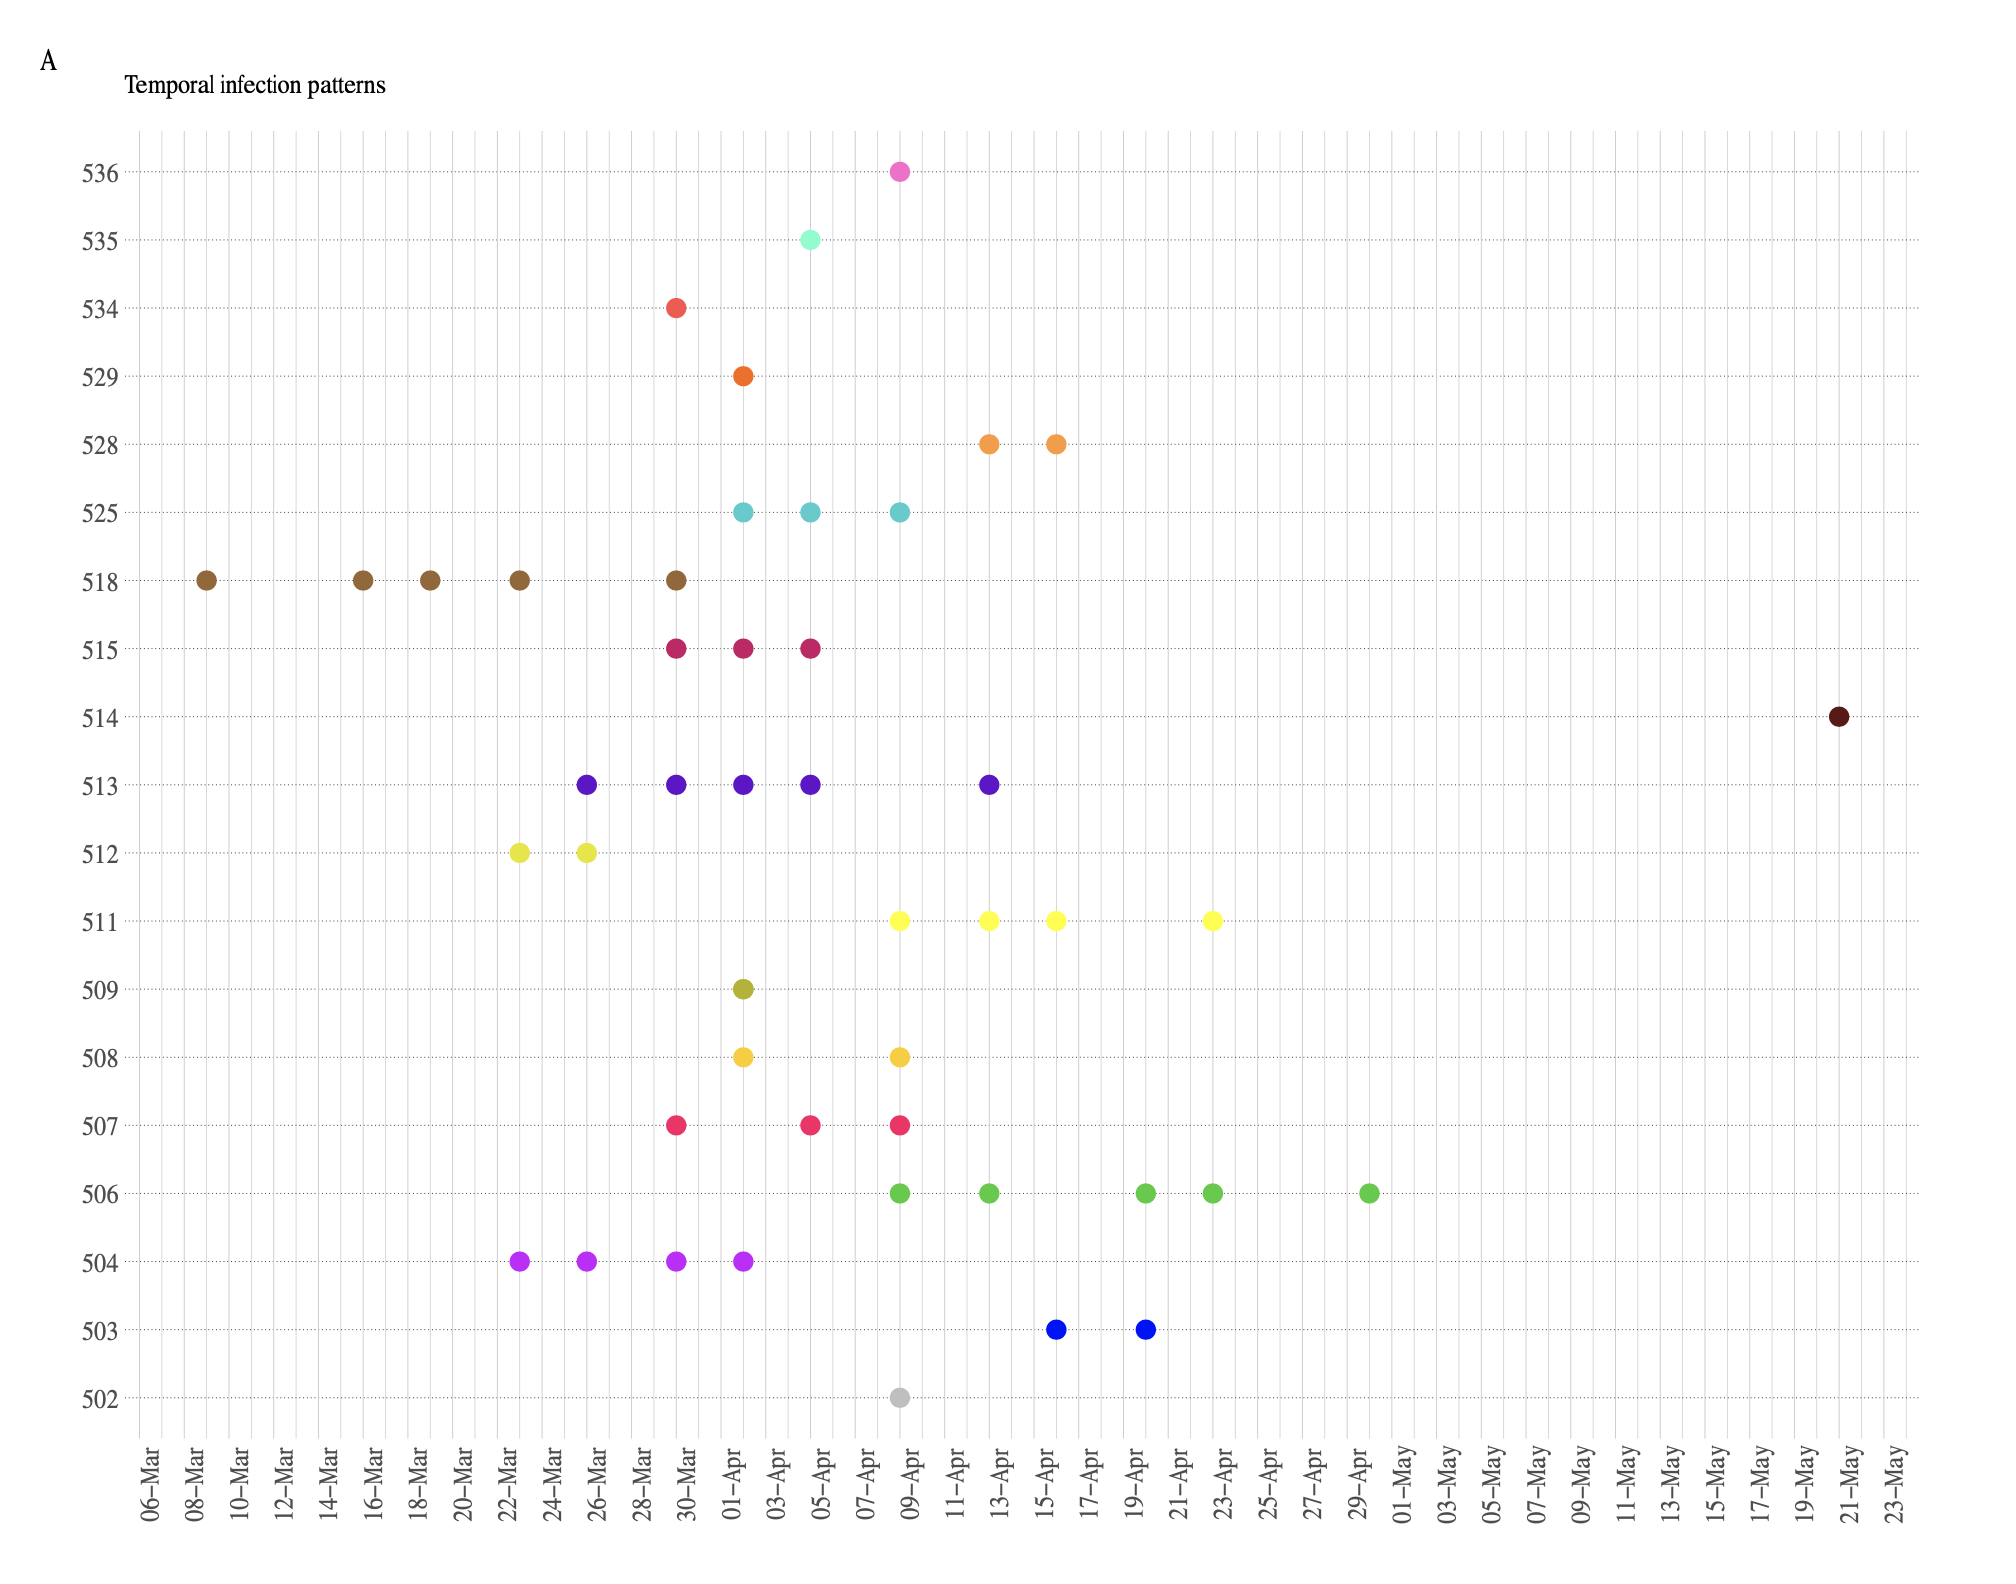
\includegraphics[width=0.75\textwidth]{../Figures/RSV/Githinji_HH_5_temporal_distribution.png}
\caption[Temporal Distribution of RSV Sample Collection]{\label{fig:orgbba1b9e}The y-axis shows anonymized individuals represented by integers and unique colors and on the x-axis is the dates on which they were sampled.}
\end{figure*}

\subsubsection{Preprocess and Quality Control}
\label{sec:org2b20197}
We started by removing reads with a Phred score below 35 and trimming sequencing
adapters as shown in \ref{sec:org6faa558} then compiled a list 
of the file paths into a text file as shown in \ref{sec:org782f498}.

Sequences in two datasets (\texttt{H\_536\_09\_04} and \texttt{H\_506\_13\_04}), specifically those 
stated \ref{sec:orgd409f8e}, caused seqwish
(\url{https://github.com/ekg/seqwish}) to crash and were therefore removed from the 
experiment leaving us with 51 samples.

\subsubsection{Construct the Assembly Graph}
\label{sec:orgaf2a392}
We used minia \cite{chikhiSpaceefficientExactBruijn2013} to construct two assembly
graphs with a k-mer length of 31 and varying minimum abundance values.
Given the nature of the dataset (51 samples of approximately 400-500 megabytes 
from a genome that is approximately 15 kilobases in length) it was clear 
that the data was noisy and we had to set a high minimum abundance. 
We varied the minimum abundance values between 1,000 and 2,000 as shown 
in \ref{sec:org54f01d2} to get a graph of size not greatly exceeding that of
the RSV genome.

A minimum abundance of 1,000 resulted in 157 kilobyte
(approximately 10x the genome size) GFA while a minimum abundance of 2,000 
resulted in a 237 kilobyte GFA (approximately 20x the genome size).
Increasing the minimum abundance from 1,000 to 2,000 reduced the size of the 
resulting graph but on visual inspection seemed to have lost some of 
the variable regions as seen in Figure \ref{fig:orgc0a4a56}.

\begin{figure*}[h]
\centering
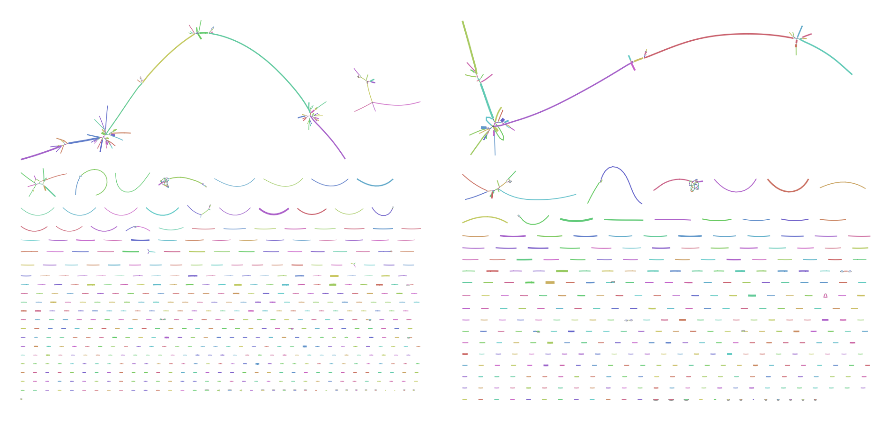
\includegraphics[scale=1.0]{../Figures/RSV/Assembly_Combined.png}
\caption[RSV Assembly Graph]{\label{fig:orgc0a4a56}An assembly graph of the household 20 samples built using minia and a minimum abundance of 1000 left and 2000 to the right.}
\end{figure*}

\subsubsection{Bluntify the Assembly Graph}
\label{sec:orgf8e04a9}
Going with the 1,000 minimum abundance graph for its increased variability but 
still manageable size we used stark (\url{https://github.com/hnikaein/stark}) to 
bluntify, that is reduce the overlaps on edges,
 \cite{gargGraphbasedApproachDiploid2018} of the graph as shown in
\ref{sec:orgd99df5b}.
This yielded a 206 kilobyte GFA that when visualized is seen in Figure
\ref{fig:org7366b45}.

\subsubsection{Prepare the Graph for Mapping with VG}
\label{sec:org7657acb}
The bash script in \ref{sec:org0bec5af} was used to chop and sort the graph
for use with vg \cite{garrisonVariationGraphToolkit2018} which led to the 
variation graph in Figure \ref{fig:org74aa235}.

\subsubsection{Mapping}
\label{sec:orgbfc4b12}
\paragraph{Convert GFA to vg Compatible Variation Graph}
\label{sec:orge74585a}
Using the instructions in \ref{sec:orge77ee86}, we induced a vg 
\cite{garrisonVariationGraphToolkit2018} compatible variation graph and output it 
GFA.

\paragraph{Index}
\label{sec:orgb859e03}
There was no need to prune the graph because it was small 
(a 62 kilobyte graph.vg) and we wanted to avoid losing complex regions such as 
those with many variants close to each other.
We, therefore, only built an index as in \ref{sec:orgc91a242} and got a 61
kilobyte graph (graph.xg) and a 258 kilobyte index (graph.gcsa).

\paragraph{Mapping}
\label{sec:org8b6399c}
To map each sample against the graph, we used \ref{sec:org4046f60} to loop through 
each of our interleaved sequences and stored the output GAM files in a 
directory of our specification.

We then verified that the alignments made sense
(a task that is both subjective and a matter of judgment) by converting the GAM 
to GAMP using the instructions in  \ref{sec:org3032d23} and viewing the JSON.

\subsubsection{Calculate Coverage Across the Graph for Each Sample}
\label{sec:org34a8932}
We used the script in \ref{sec:orgc85b3b9} to generate a coverage vector 196,488 nodes
long in tsv (tab separated values) format.

\subsubsection{Normalization}
\label{sec:org33e9040}
The coverage data had a lot of outliers, as shown in Figure
\ref{fig:org68a928c}, and therefore needed normalization to avoid the outliers
skewing it.

\begin{figure*}[h]
\centering
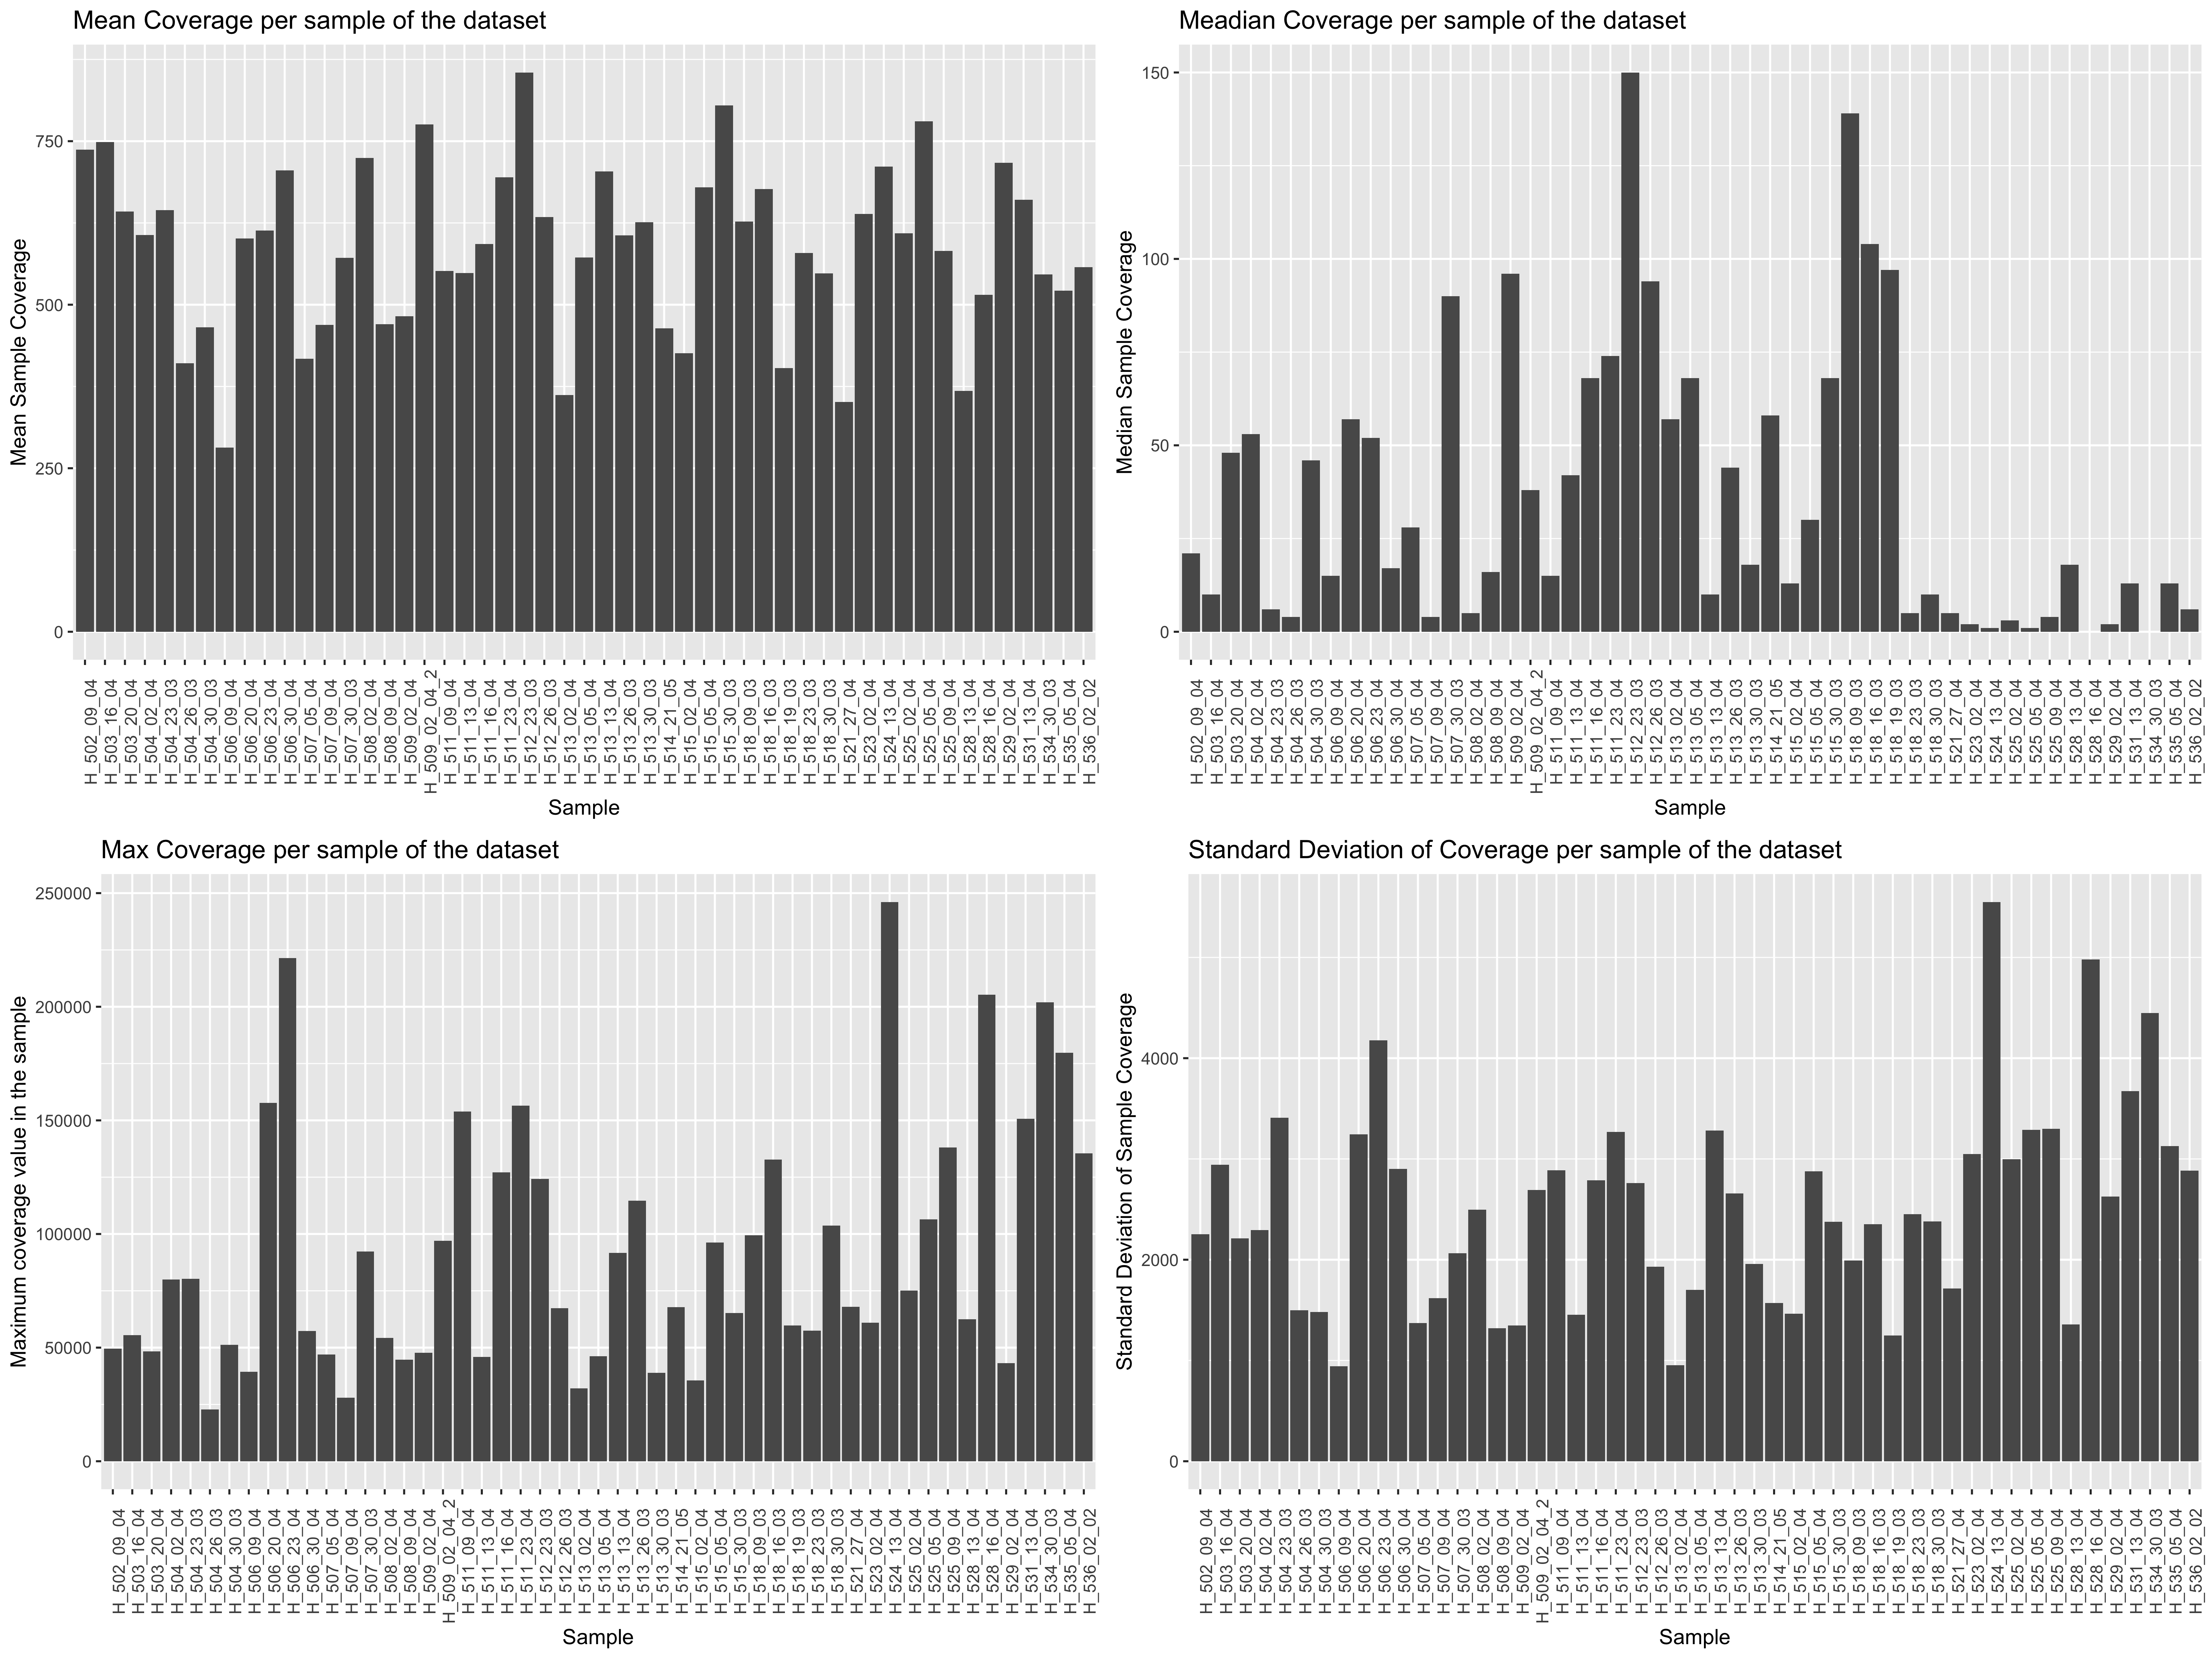
\includegraphics[width=0.75\textwidth]{../Figures/RSV/structure_of_coverage_data.png}
\caption[RSV Structure of the Data]{\label{fig:org68a928c}Bar graphs of mean, median, maximum and standard deviation of coverage values per sample}
\end{figure*}


We normalized the coverage by setting any coverage value above zero as one and 
left the zero values as zero. This meant that in this analysis, any form of
coverage no matter how deep was valued equally which yielded the heatmap in
Figure \ref{fig:org4444337}.

\begin{figure*}[h!]
\centering
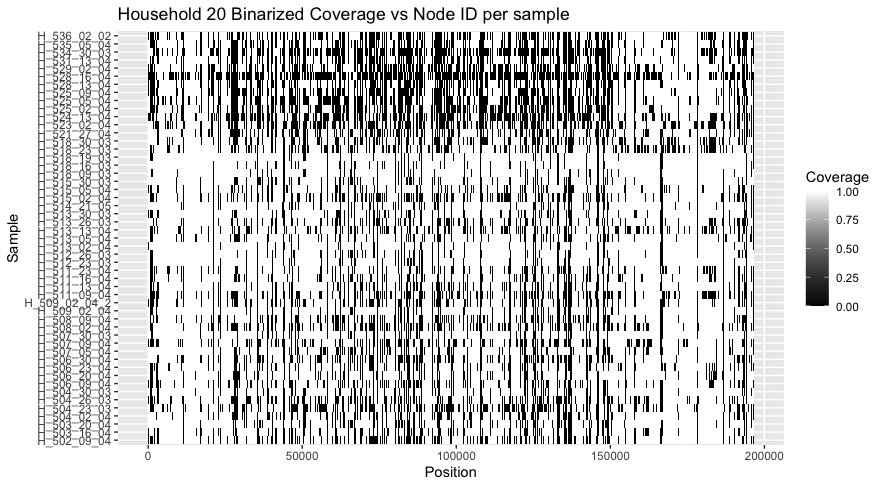
\includegraphics[width=0.7\textwidth]{../Figures/RSV/Heatmap.png}
\caption[RSV heatmap]{\label{fig:org4444337}A heatmap of the binary normalized coverage vectors of the forty nine RSV samples. On the x axis is the node identifier and the y axis are the individual samples. The light regions indicate coverage while the dark regions indicate no coverage.}
\end{figure*}

\newpage
\subsubsection{Principal Component Analysis}
\label{sec:org0b369bb}
To make it possible to compare the high dimensional data, we applied Principal 
Component Analysis (PCA) which was able to differentiate each of the samples.
Figure \ref{fig:orga05c68e} is a scatter plot of the first and second principal 
components for RSV reads.

\begin{figure*}[h]
\centering
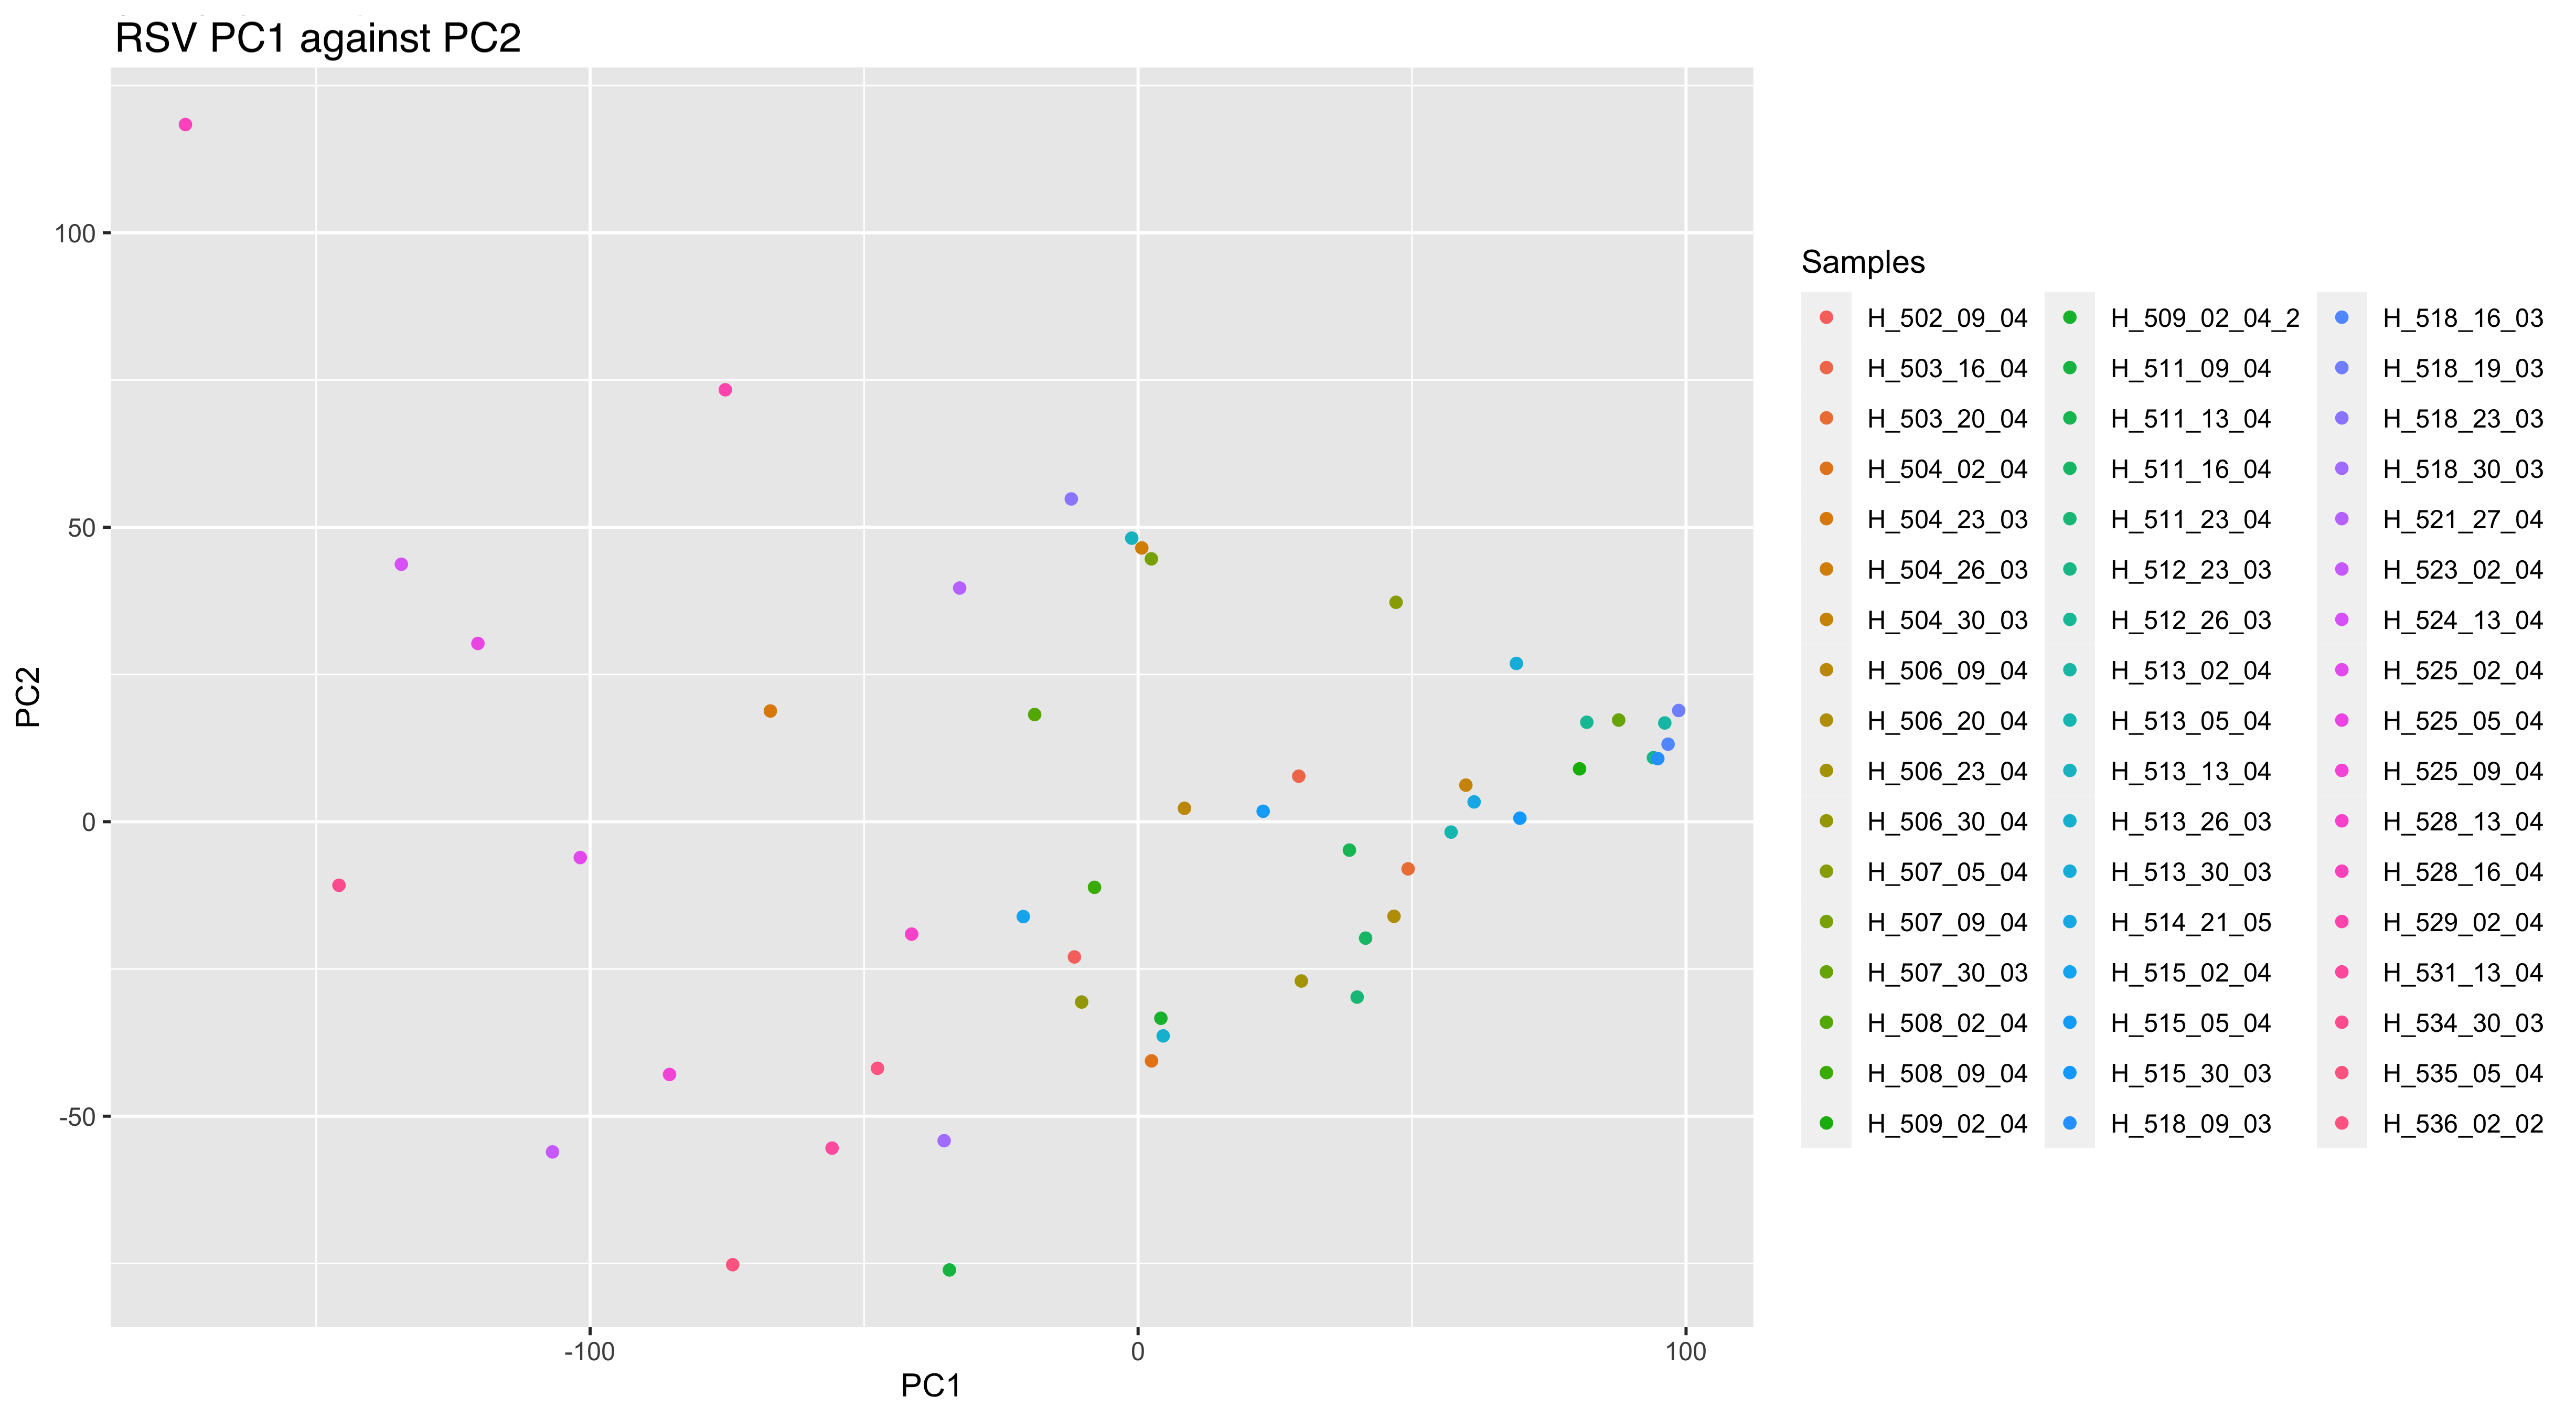
\includegraphics[width=0.75\textwidth]{../Figures/RSV/PCA.png}
\caption[RSV PCA]{\label{fig:orga05c68e}A scatter plot of the first and second principal components of the coverage vectors of the forty nine RSV samples.}
\end{figure*}


\begin{figure*}[h]
\centering
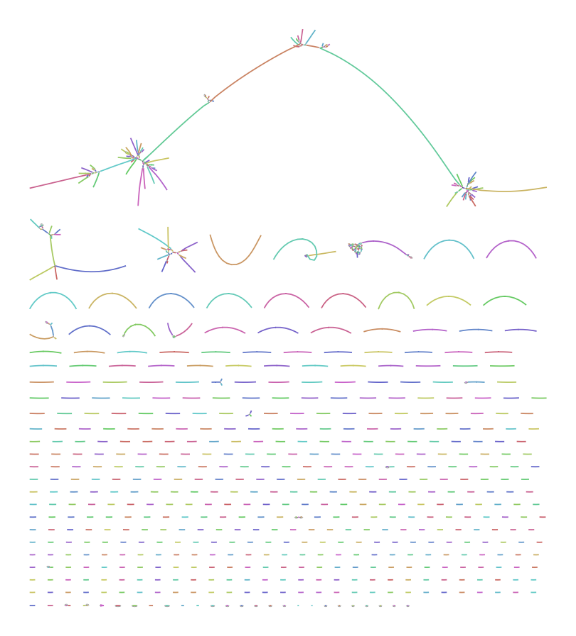
\includegraphics[width=0.75\textwidth]{../Figures/RSV/Assembly_Bluntified.png}
\caption[Bluntified RSV Assembly Graph]{\label{fig:org7366b45}RSV household 20 assembly graph bluntified using stark.}
\end{figure*}

\begin{figure*}[h!]
\centering
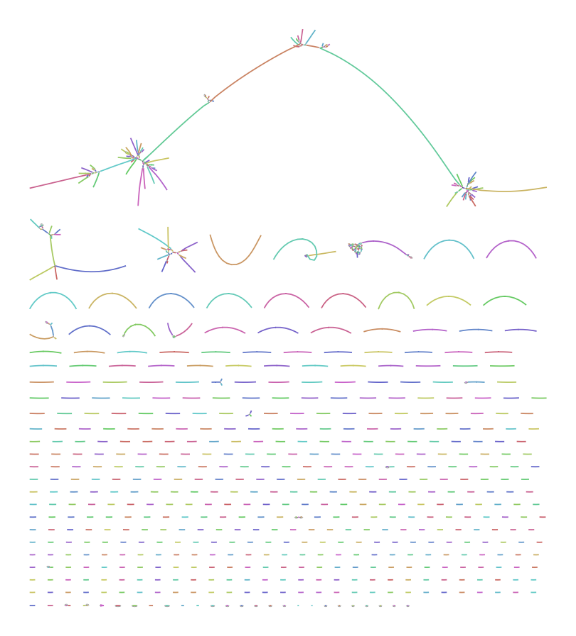
\includegraphics[width=0.75\textwidth]{../Figures/RSV/Assembly_Bluntified.png}
\caption[RSV Variation Graph]{\label{fig:org74aa235}The household 20 variation graph after running odgi chop on it.}
\end{figure*}

\clearpage

\clearpage
\section{Results}
\label{sec:org566bae9}
Using the distances matrix, we were able to cluster closely related samples
together inferring this relatedness based on how they mapped to the graph. 

The infant in the household was member 502 from whom only a single sample was
sequenced. Hierarchical clustering of household dataset, zoomed in in
Figure \ref{fig:orgb4d4cf6}, shows that member 506 had the earliest closest sample
to that of the infant 502 and 528.
The closest sample to the infant is from member 528.
We also see that member 518, a school going eleven year old, has their samples
sit on their own.
Also interesting to note is member 508, a two-year-old, had their sample cluster
very closely to that of the infant.

\begin{figure*}[h]
\centering
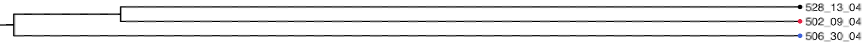
\includegraphics[width=1.0\textwidth]{../Figures/hh20-clado-infant.png}
\caption[A section of the cladogram of RSV focused on the infant]{\label{fig:orgb4d4cf6}Hierarchical clustering of simulated RSV focusing on member 502, the infant.}
\end{figure*}


When it comes to the entire household, the cladogram in Figure \ref{fig:org3ca3c54} shows three
clades circulating in household five annotated using red, blue and green rectangles.
In terms of when samples were taken, it is interesting to note that all but one
(504) of the samples collected in March cluster together in the clade
highlighted in red while the samples collected in April cluster in the clades
annotated in blue and green.

It is worth noting that despite only showing a rooted tree, both rooted and
unrooted neighbour trees can be generated by this method.

\begin{figure*}
\centering
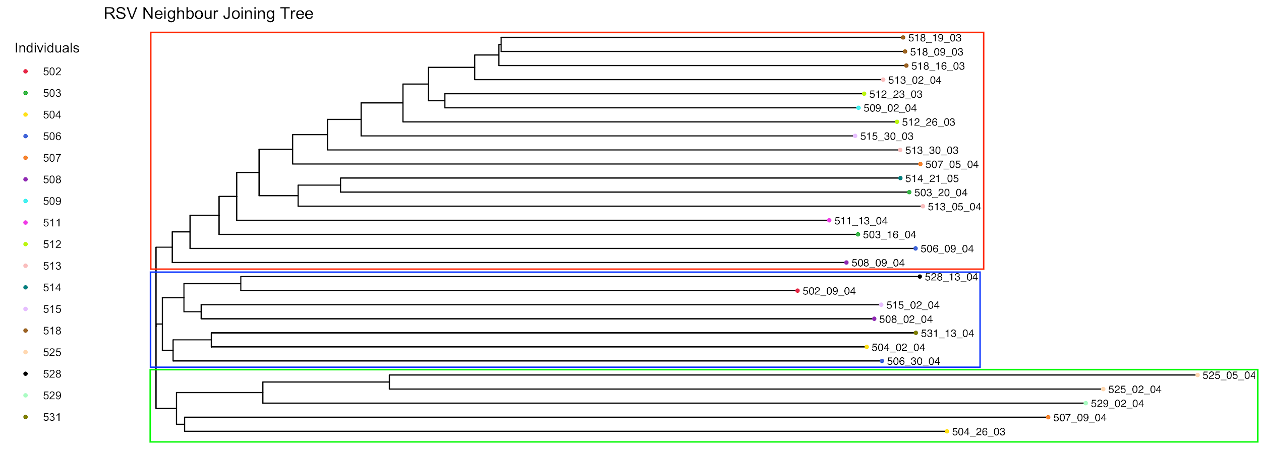
\includegraphics[width=1.0\textwidth]{../Figures/hh20-clado.png}
\caption[A cladogram of RSV]{\label{fig:org3ca3c54}A cladogram of the Household five dataset generated by neighbour-joining of the distance matrix of its coverage vector.}
\end{figure*}
\newpage
\section{Discussion}
\label{sec:org9b13229}
The study set out to establish whether comparing samples based on how their
sequence reads aligned to a reference graph provides sufficient resolution to
understand who infects the infant with RSV in the household.
It found that by mapping sequence reads to a reference genome graph, we gain
high enough resolution to differentiate and cluster samples in the household.
We are therefore performing an all vs all sample comparison through a
representative proxy, coverage against a graph.
It is also worth noting that using this method, we were able to differentiate
samples better than the tools used in previous studies.
The study did not go far enough to try and establish transmission chains in the
household or the circulation of different subtypes and genotypes, but that does
not mean that it is not possible.

Contemporary methods of reference genome representation use a linear model, a
golden path, to represent a shared genome and a separate file to hold variation
information such as a VCF file leading to a failure to account for some of the
genetic variations during mapping.
This model is lossy as a result of its linearity because it is a consensus of
the most frequently occurring sequences amongst the sequences used to build it.
The lack of lower frequency variants, in turn, causes the model to favour
high-frequency variants leading to a tendency to over-report sequences present
in the reference and under-report those that are not.
This tendency, known as reference allele bias, leads to an underestimation of
the genetic variation present in a genome. Moreover, the reference is not
transitive (\(A>B\ and\ B>C,\ therefore,\ A>C\)) and therefore not an ideal way to compare samples.
That is, how a sample  compares to reference and how another sample  compares to
the reference does not mean that it is possible to conclusively compare  against
based on how they compare against the reference.

Graph-based models sidestep the lack of transitivity problem by being able to
present alternatives and when used to represent the reference genome have been
shown to reduce reference allele bias, consequently facilitating the comparison
of genomes at a higher resolution than before.

When it comes to who infects whom in the household; the premise of this work is
that sample relatedness is a proxy for transmission.
I expect a person to have a virus that is genetically similar to that of the
people the person infects. Therefore, infections of similar origin will cluster
together because like samples will cluster together.

We find all one but one (504) of the samples collected in March cluster together
in the clade highlighted in red while the samples collected in April cluster in
the clades annotated in blue and green. It is also fascinating to see that
member, 518, a school going eleven years old, has their samples sit on their
own, implying they did not acquire their RSV infection from a member of the
household. This is very interesting and expected because it shows that samples
collected at around the same time were genetically similar.
It also shows that the samples from the school going child were consistently
different from the others.

It is highly likely that the individual whose sample clustered closest to that
of the infant could have been the ones who transmitted the virus to the infant.
In this case, the two-year-old, 528, had their sample sit closest to that of the
infant, implying that the infant's RSV infection is from the two-year-old.

\subsection{Strengths and limitations}
\label{sec:org716aacd}
Genome graphs give insight into genetic variation in ways that are not possible
with existing tools.
It was possible to come up with an intuitive method, useful for comparing
samples through the aid of genome graphs which provide a higher resolution when
looking at pangenomes or in our case a virus quasispecies. By representing
alternative bases, aligning reads against these alternative bases, and then
analysing the coverage of these alignments, it is possible to analyse genomes at
a higher resolution than the methods that make use of linear references do.

This study did not attempt to differentiate between genotypes and subtypes of
RSV or investigate and how they circulate within the household.
It is also not entirely conclusive and uses a naive approach that does not
account for noise or the varying level of significance between mapping to a
given node versus another.

\newpage
\section{Conclusion}
\label{sec:orgfd1d29b}
This thesis does not expressly state the two-year-old transferred RSV to the
infant, but it does show that the two-year-olds sample was most related to that
of the infant.
Meaning genome graphs provide enough resolution to cluster RSV samples in the
household in ways that the methods used in previous studies could not. 

The study presents an intuitionistic and straightforward approach of comparing
samples.
This approach facilitates an all versus comparison of samples without going
through the linear reference as is the norm and possibly avoiding the
transitivity issue.
Using the depth of coverage under each node; it is possible to generate
cladograms through neighbour-joining and hierarchical clustering.
This method was able to split the household RSV dataset into three different
clades; a task that proved difficult with methods based on linear references.

To investigate the circulation of subtypes and genotypes of RSV
(or any other virus) I propose two ways to go about it: one, a reference graph
for each subtype or genotype or two, a pangenome graph for RSV with the nodes
containing bases that are specific to given subtypes annotated.
Determining whether a genotype or subtype is present in a sample would be a
matter of checking whether the reads that map to a type-specific graph or a
subgraph of a pangenome graph reach a set threshold.

Future work will involve verifying that these cladograms are differentiating
these samples correctly and how it compares to contemporary methods of
phylogenetics.
It would also be interesting to see what statistical noise reduction or
dimensionality reduction techniques could do to the coverage vector.
It is also possible to use techniques other than the euclidean distance to
analyse the coverage data. Moreover, it would be desirable to have a world in
which it is possible to look up a new sample's coverage against an already
trained model.

\newpage
\bibliographystyle{apacite}
\bibliography{../library}

\begin{appendices}
\subsection{Code}
\label{sec:org5bddd28}

\subsubsection{Quality Control and Adapter Trimming}
\label{sec:org6faa558}
\begin{verbatim}
# concatenate the contents of all the files
# in ~/miniconda3/share/trimmomatic-0.39-1/adapters/ into one
# file, in my case adapters.fa and use those to trim adapters

trimmomatic PE \
 data/H_528_16_04/H_528_16_04_1.fastq.gz \
 data/H_528_16_04/H_528_16_04_2.fastq.gz \
 trimmed_forward_paired.fq.gz trimmed_forward_unpaired.fq.gz \
 trimmed_reverse_paired.fq.gz trimmed_reverse_unpaired.fq.gz \
 ILLUMINACLIP:adapters/adapters.fa:2:35:10:2:keepBothReads \
 SLIDINGWINDOW:4:35
\end{verbatim}

\subsubsection{Concatenate Reads into Text File}
\label{sec:org782f498}
\begin{verbatim}
find $(pwd)/data -d -name '*interleave*fq' > sequences.txt
\end{verbatim}

\subsubsection{Problematic RSV Sequences}
\label{sec:orgd409f8e}
\begin{verbatim}
data/H_536_09_04/H_536_09_04_interleaved.fq:1271846:AGAACTCAGTGTAGGTAGAATGGTTGGCTGATCAATATCTCTAATGATTTTGGTCTGTGAATCAACTGTCATAAGAGAATTCTATCAAAGTTGAATTCCGAATCCTTGGGTCAATGACTGGGTGCACCCATTCTTCTAATGTGCTCTGTC
data/H_506_13_04/H_506_13_04_interleaved.fq:3831798:AGAACTCAGTGTAGGTAGAATGGTTGGCTGAGTAGGTAGATGGAGGCAGGTGCATGTGTGATGGGAAGTGTGGTGACGGGTTGTGTGGGCACACGGGATGAGGCGCAGATGGCTGGGGGTTTGGGAGGGGAATGGGTGGGAGAAGGAGGC
\end{verbatim}

\subsubsection{Minia Fragment Assembly}
\label{sec:org54f01d2}
\begin{verbatim}
minia -in ../sequence_paths.txt \
  -kmer-size 31 \
  -abundance-min 1000 \
  -nb-cores 8
\end{verbatim}

\subsubsection{Graph Bluntification Using Stark}
\label{sec:orgd99df5b}
\begin{verbatim}
stark -i input_file_name \
  -o stark_bluntify.gfa \
  -s cpu-consuming
\end{verbatim}

\subsubsection{Odgi Graph Preparation}
\label{sec:org0bec5af}
\begin{verbatim}
#!/usr/bin/env bash

# premap.sh

InputGFA=$1
BuildVG="build-odgi.vg"
ChoppedVG="chopped-odgi.vg"
SortedVG="sorted-odgi.vg"
ViewGFA="view-odgi.gfa"

echo "Using $InputGFA"
odgi build \
     -s \
     -g ${InputGFA} \
     -o ${BuildVG}

echo "Chopping to size 1024"
odgi chop \
     -i build-odgi.vg \
     -c 1024 \
     -o ${ChoppedVG}

echo "Sorting"
odgi sort \
     -i chopped-odgi.vg \
     -o ${SortedVG}

echo "Generating GFA $ViewGFA"
odgi view \
     -i sorted-odgi.vg \
     -g \
     > ${ViewGFA}

# Run with
./pre-map.sh stark_bluntify.gfa
\end{verbatim}

\subsubsection{RSV VG View}
\label{sec:orge77ee86}
\begin{verbatim}
vg view -Fv view-odgi.gfa > graph.vg
\end{verbatim}

\subsubsection{RSV VG Index}
\label{sec:orgc91a242}
\begin{verbatim}
vg index -x graph.xg -g graph.gcsa graph.vg
\end{verbatim}

\subsubsection{RSV VG Map Script}
\label{sec:org4046f60}
\begin{verbatim}
#!/usr/bin/env bash

Graphname="graph"
# Using a gams dir to put the gam files
GAMDir="gams"

# For each file in the sequence list, call vg to map it to the graph
while read Filepath;
do
    # paramter expansion http://mywiki.wooledge.org/BashFAQ/073
    Filename=${Filepath##*/}
    FileStub=${Filename%_*}

    echo "Mapping $FileStub"
    vg map \
       -f ${Filepath} \
       -x ${Graphname}.xg \
       -g ${Graphname}.gcsa \
       > ${GAMDir}/${FileStub}.gam

# Run with
./map.sh < ../sequence_paths.txt
\end{verbatim}

\subsubsection{Generate GAM}
\label{sec:org3032d23}
\begin{verbatim}
vg view -a -k gams/H_513_02_04.gam > Images/H_513_02_04.gamp
vg view -K -j Images/H_513_02_04.gamp > Images/H_513_02_04_GAMP.json
cat Images/H_513_02_04_GAMP.json | jq | less
\end{verbatim}

\subsubsection{VG Pack Script}
\label{sec:orgc85b3b9}
\begin{verbatim}
#!/usr/bin/env bash

# Loop through each gam file
Graphname="graph"
CoverageDir="coverage"

while read Filepath;
do
    # parameter expansion http://mywiki.wooledge.org/BashFAQ/073
    FileStub=${Filepath%.*}

    vg pack \
       -d \
       -x ${Graphname}.xg \
       -g ${Filepath} \
       > ${CoverageDir}/${FileStub}.pack.table
done

# Run with

find $(pwd)/gams -d -name '*.gam' > gams.txt
./map.sh < gams.txt
# or
./coverage.sh < find $(pwd)/gams -d -name '*.gam'
\end{verbatim}
\end{document}
